%%%%%%%%%%%%%%%%%%%%%%%%%%%%%%%%%%%%%%%%%%%%%%%%%%%%%%%%%%%%%
% Preamble Options
%%%%%%%%%%%%%%%%%%%%%%%%%%%%%%%%%%%%%%%%%%%%%%%%%%%%%%%%%%%%%

% Select build mode from:
%     quick - try to compile quickly (no extras, remove front pages)
%     debug - add grid lines/compile times (print variables)
%     proof - local version of "final"
%     final - Final publishable version (calls PurdueThesis - requires LuaLaTeX)
\def\ZZbuildmode{final}

% Input arguments required by PurdueThesis

% ----------------- Author/Document Info -----------------
% Auuthor Name
\def\ZZauthor{Sesha Charla}

% "May XXXX", "August XXXX", or "December XXXX"
\def\ZZgraduation{December 2025}

% Title
\def\ZZtitle{Model based FDI and Reconfiguration using Set Membership and Adaptive Robust Control Techniques}


% -------------------- Degree Program ---------------------
% Either:
%     Doctor of Philosophy
%     Master of Science in Aeronautics and Astronautics
\def\ZZdegree{Doctor of Philosophy}

% Either "A Dissertation" or "A Thesis"
\def\ZZdocument{A Preliminary Report}


% --------------- Final Draft Defaults (AAE) ---------------

% Purdue AAE (West Lafayette)
\def\ZZinstitution{Purdue University}
\def\ZZcampus{West\space Lafayette}
\def\ZZprogram{Mechanical Engineering}

% Defaults for final draft
%      These are overwritten in PurdueThesisNL.cls but
%      not in PurdueThesis.cls
\def\ZZshowgridlines{false}
\def\ZZshowmarginlines{false}
\def\ZZshowtimestamp{false}
\def\ZZtodonotes{false}
\def\ZZatinformation{}
\def\ZZshowcolophon{false}
\def\ZZshowdiagonalline{false}


% Build the document this will select the document class based on :
%    quick/debug/proof - Local simplified PurdueTheiss.cls file
%                final - Official PurdueThesis.cls file
\RequirePackage{ifthen}
\ifthenelse{\equal{\ZZbuildmode}{final}}
{\documentclass{PurdueThesis}}{\documentclass{PurdueThesisNL}}

% Set up the latex document w/ imports, definitions, and
% template customizations
\ConfigureBibliography
% \graphicspath{{eps/}{tiff/}}
\graphicspath{{figures/}{figures/template}}

% Look in the "packages" subfolder for packages.
% This is done to reduce the number of files in the main thesis folder
% so the ones in there are easier to find.
\makeatletter
  \def\input@path{{packages/}}
\makeatother

% The vertical space between a table heading and the table contents in a tabular environment.
\newcommand{\tabularspace}{\noalign{\vspace*{2pt}}}

% Define boolean variables that contorl how the document is compiled
\newboolean{quick}
\newboolean{debug}
\newboolean{proof}
\newboolean{final}
\newboolean{quick-or-debug}
\newboolean{proof-or-final}

\ifthenelse{\equal{\ZZbuildmode}{quick}}
    {\setboolean{quick}{true}}{\setboolean{quick}{false}}
\ifthenelse{\equal{\ZZbuildmode}{debug}}
    {\setboolean{debug}{true}}{\setboolean{debug}{false}}
\ifthenelse{\equal{\ZZbuildmode}{proof}}
    {\setboolean{proof}{true}}{\setboolean{proof}{false}}
\ifthenelse{\equal{\ZZbuildmode}{final}}
    {\setboolean{final}{true}}{\setboolean{final}{false}}

\ifthenelse{\boolean{quick} \OR \boolean{debug}}
  {\setboolean{quick-or-debug}{true}}
  {\setboolean{quick-or-debug}{false}}
\ifthenelse{\boolean{proof} \OR \boolean{final}}
  {\setboolean{proof-or-final}{true}}
  {\setboolean{proof-or-final}{false}}

% -------------------- From Template -------------------

% So "_" will work in URLs when using BibTeX.
\usepackage[T1]{fontenc}

% The mathtools package
% (see http://mirror.utexas.edu/ctan/macros/latex/required/amsmath/amsmath.pdf)
% loads the amsmath package which defines the
%     align
%     align*
%     alignat
%     alignat*
%     equation
%     equation*
%     flalign
%     flalign*
%     gather
%     gather*
%     multitaper
%     multitaper*
%     split
% environments and extends amsmath by defining many other commands.
% See
%     https://ctan.org/pkg/amsmath
% for information about amsmath and
%     http://ctan.math.washington.edu/tex-archive/macros/latex/contrib/mathtools/mathtools.pdf
% for information about mathtools.
\usepackage{mathtools}

% Define \FigureDash.
% \FigureDash is a dash the width of a digit in the current font.
\usepackage{pa-figure-dash}

% For PurdueThesis, PuTh, TeX, LaTeX, METAFONT, METAPOST, etc. related logos.
\usepackage{pa-logos}

% (Or maybe use isomath instead?  -mark  2021-06-20)
% Follow ISO 80000-2:2019
%     o   put e, i, j, and pi in upright font automatically
%     o   use, for example, "\di x" to get "\,mathrm{d}\/x"
% This loads
%     o   amsmath.sty (which is already loaded above)
%     o   mathtools.sty
%     o   upgreek.sty
% Load the package.
\usepackage{pa-mismath}
    % Tell mismath to put e, i, j, and pi in upright font automatically.
    \enumber
    \inumber
    \jnumber
    \pinumber
  % To typeset math italic e, i, j, and pi use
  %     \mathit e
  %     \mathit i
  %     \mathit j
  %     \itpi


% Define \FloatBarrier
\usepackage{placeins}

% For highlighting text using \hl
\usepackage{soul}

% For \sfrac, used to do slanted fractions, similar to, e.g., 1/2, but 1 is small and high and 2 is small and low.
\usepackage{xfrac}

% For typographical conventions stuff including
%     \Emph{...}
%     \First{...}
%     \Keys{...}
%     \Literal{...}
%     \Menu{...}
%     \Place{...}
%     \Shell{...}
% This must be after
%     \usepackage{tikz}
\usepackage{pa-typographic-conventions}


% ----------------- Added Dependencies -----------------

% Generate lorem ipsum 
%    e.g.: \lipsum[1-2]
\usepackage{lipsum}

% To sort variables alphabetically in debug mode
\usepackage{datatool}

% Extra math symbols
%     mathbb
\usepackage{amssymb}

% Acronyms
\usepackage[acronym]{glossaries}
  \glsdisablehyper

% cleveref
%   For easier cross-referencing
%   Redefine the subref formatting so that you get:
%     Figure 1.1(a) instead of Figure 1.1a
\usepackage[noabbrev, capitalise]{cleveref}
  \captionsetup[subfigure]{subrefformat=simple,labelformat=simple}
  \renewcommand\thesubfigure{(\alph{subfigure})}

% Put table captions on top / adjust the spacing
\captionsetup[table]{
    position=above,
    belowskip=4pt
  }


% Define \NL (newline) so LaTeX goes to the next output line.
% Just doing \\ complains
%     ! LaTeX Error: There's no line here to end.
% \mbox{} is an empty math box.
\newcommand{\NL}{\mbox{}\\}



% To keep track of variables used in the document
%    for optional printing when in debug mode
\makeatletter
    \newcommand*\paperVariables{}
    \newcommand*\paperSortVars{}
    \newcommand*\storeVariables[2]
    {\ifx\paperVariables\empty
        \def\paperVariables{{#1,#2}}%
    \else
        \g@addto@macro\paperVariables{, {#1,#2}}%
    \fi
    }
    \makeatother
    

% Use \varDef instead of \newCommand to track variables for debug mode
%       #1: latex command for the variable (e.g. \myAngle)
%       #2: symbol to use (e.g. a, A, \alpha)
%       #3: (optional) font class (e.g. \mathbb )
\def\temp{ \NewDocumentCommand{\varDef}{m m o e{_^}} }

\ExplSyntaxOn
\temp{%
    \IfValueTF{#3}{ %
        \newcommand{#1}{{#3{#2}}\IfValueT{#4}{\sb{#4}}\IfValueT{#5}{\sp{#5}}}%
    }{%
        \newcommand{#1}{{#2}\IfValueT{#4}{\sb{#4}}\IfValueT{#5}{\sp{#5}}}%
    }%
    % \IfValueT{#5}{^{#5}}%
    % Only store variables if needed for debug mode
    \ifthenelse{\equal{debug}{\ZZbuildmode}} { %
        \storeVariables{#1}{#2}}{} %
} %
\ExplSyntaxOff


% Vector formatting
\newcommand{\vectorFmt}[1]{\pmb{#1}}
\newcommand{\unitVecFmt}[1]{\hat{#1}}
\newcommand{\sub}[2]{{#1}_{#2}}
\newcommand{\upRight}[2]{{#1}^{#2}}
\newcommand{\upLeft}[2]{{}^{#2} {#1}}
\newcommand{\firstDerivative}[1]{\dot{#1}}
\newcommand{\secondDerivative}[1]{\ddot{#1}}

% Define useful variables of the form:
%    \vardef{\command}{var-name}[\format] 

% Testing out some basic ones
\varDef{\zNd}{z}
\varDef{\xNd}{x}
\varDef{\yNd}{y}
\varDef{\xDim}{X}
\varDef{\yDim}{Y}
\varDef{\zDim}{Z}
\varDef{\angleTwo}{\beta}
\varDef{\angleOne}{\alpha}
\varDef{\angleFour}{\Pi}
\varDef{\angleThree}{\Gamma}
\varDef{\otherCvar}{C}
\varDef{\nBody}{N}

% Math
\varDef{\Real}{R}[\mathbb]
\varDef{\Complex}{C}[\mathbb]

% Stats
\varDef{\Normal}{N}[\mathcal]
\varDef{\Uniform}{U}[\mathcal]
\varDef{\ExpVal}{E}[\mathbb]

% Dynamical Systems
\varDef{\lagrangian}{L}[\mathcal]
\varDef{\hamiltonian}{H}[\mathcal]

% To show how formatting is handled
\varDef{\vectorFormat}{x}[\vectorFmt]
\varDef{\unitVectorFormat}{x}[\unitVecFmt]

% How about superscripts?
\varDef{\xSquared}{x}^{2}
\varDef{\xSubTwo}{x}_{2}
\varDef{\xSubTwoSquared}{x}_{2}^{2}
\varDef{\aVectorSquared}{y}[\vectorFmt]^{2}

% Tableau Colors (Matplotlib Defaults)
\definecolor{tab-blue}{HTML}{1F77B4}
\definecolor{tab-orange}{HTML}{FF7F0E}
\definecolor{tab-green}{HTML}{2CA02C}
\definecolor{tab-red}{HTML}{D62728}
\definecolor{tab-purple}{HTML}{9467BD}
\definecolor{tab-brown}{HTML}{8C564B}
\definecolor{tab-pink}{HTML}{E377C2}
\definecolor{tab-gray}{HTML}{7F7F7F}
\definecolor{tab-yellow}{HTML}{BCBD22}
\definecolor{tab-cyan}{HTML}{17BECF}

% See https://marcom.purdue.edu/our-brand/visual-identity
%   and https://marcom.purdue.edu/app/uploads/2020/01/AA_ColorChart_NEW_BRAND.pdf
\definecolor{purdue-boilermaker-gold}{HTML}{cfb991}
\definecolor{purdue-aged}{HTML}{8e6f3e}
\definecolor{purdue-rush}{HTML}{daaa00}
\definecolor{purdue-field}{HTML}{ddb945}
\definecolor{purdue-dust}{HTML}{ebd99f}
\definecolor{purdue-steel}{HTML}{555960}
\definecolor{purdue-cool-gray}{HTML}{6F727B}
\definecolor{purdue-railway-gray}{HTML}{9d9795}
\definecolor{purdue-steam}{HTML}{c4bfc0}
\newacronym{nrho}{NRHO}{Near Rectilinear Halo Orbit}
\newacronym{crtbp}{CR3BP}{Circular Restricted Three Body Problem}
% TODO: not sure if everything should use \input

%%%%%%%%%%%%%%%%%%%%%%%%%%%%%%%%%%%%%%%%%%%%%%%%%%%%%%%%%%%%%
% Ducument
%%%%%%%%%%%%%%%%%%%%%%%%%%%%%%%%%%%%%%%%%%%%%%%%%%%%%%%%%%%%%
\input{ltx_core/ltx_pkgs.tex}
\input{ltx_core/lst_style.tex}
\input{ltx_core/new_cmds.tex}
\bibliography{Part3/scr_refs, Part2/drone_refs, Part1/theory_refs}

\begin{document}
\maketitle

% Only include these sections if this is a proof or final version
\ifthenelse{\boolean{quick}}{}{
    % Statement of Thesis/Dissertation Approval Page
% This page is REQUIRED.  The page should be numbered "2"
% and should NOT be listed in your TABLE OF CONTENTS.

\begin{statement}
    % Delete or add \entry commands as needed for all committe members.
    \entry{Dr.~Bin Yao, Co-chair}{School of Mechanical Engineering}
    \entry{Dr.~Peter H. Meckl, Co-chair}{School of Mechanical Engineering}
    \entry{Dr.~Richard M. Voyles, Co-chair}{Polytechnic Institute}
    \entry{Dr.~George T.C. Chiu}{School of Mechanical Engineering}
    % There should be one \approvedby command containing the
    % "FORM 9 THESIS FORM HEAD NAME HERE" (from TEMPL, retrieved on 2020-03-01).
    \approvedby{Dr.~Nicole Key}
\end{statement}

    % Dedication page is optional.
% A name and often a message in tribute to a person or cause.
% References: WEB9 332.

% \ifthenelse{\boolean{quick-or-debug}}{}
% {
% \begin{dedication}
%
% \end{dedication}
% }

    % Acknowledgements page is optional but most theses include
% a brief statement of appreciation or recognition of special
% assistance.
\ifthenelse{\boolean{quick-or-debug}}{}
{
\begin{acknowledgments}
        The author acknowledges and gratefully appreciates the constant support and guidance provided by the three co-advisors, Prof. Bin Yao, Prof. Richard Voyles and, Prof. Peter H. Meckl. Prof. Voyles for providing the hardware, lab space and guidance on developing a workable research problem related to Dexterous Hexrotor and also on dealing with the problems related to hardware and software debugging. Thanks to Prof. Meckl for his consistent guidance and inspiration in development of research problem on SCR-ASC modelling and diagnostics, and supporting the author with funding in form of Research Asssitantships since the last 1.5 years. Finally, thanks to Prof. Bin Yao for training and advising the author in control theory and the constant guidance and inspiration on bringing both the research endeavors under the same umbrella.
\end{acknowledgments}
}

    % The preface is optional.
% References: TCMOS17 1.49, WEB9 927.

% \begin{preface}
%   This is the preface.
% \end{preface}
    %
    \setcounter{tocdepth}{1}
    \pdfbookmark{TABLE OF CONTENTS}{Contents}
    \tableofcontents
    \listoftables
    %\listoffigures
}

% Optional: Symbols, Abbreviations, Nomenclature, Glossary

% Always include the abstract
\begin{abstract}%

\end{abstract}


% For the official template
\setcounter{tocdepth}{1} % Might need this for the official template?
\ifthen{\equal{\ZZbuildmode}{final}}{\setcounter{tocdepth}{1}}
  % Front matter (title, acknowledgements, abstract, etc)
%%======================================================================================================================

\part{\large Theory}
%\chapter{Introduction}
The economical and safety related reasons had spurred ever-increasing interest in the theory and applications of
model-based fault detection and diagnosis methods. The use of parameter estimation techniques for fault detection of
mechanical systems was first demonstrated in \cite{baskiotis1979parameter}, \cite{geiger1982monitoring}
\cite{filbert1982quality}, \cite{hohmann1977automatic}. This as a part of larger class of fault detection based on
analytical redundancy. The development of process fault detection methods based on modelling, parameter and state
estimation was summarized by \cite{isermann1984process}, \cite{isermann1997trends}. Parity equation-based based methods
were treated early in \cite{chow1984analytical} and then later developed by Patton and others in \cite{patton1991review}
and \cite{hofling1994detection}.

Basic terminology related to fault diagnosis can be found in \cite{hofling1994detection} and \cite{ding2005model}. The following terms need specific attention:

\begin{itemize}
        \item \itbf{Fault Detection}: Determination of faults present in the system at the time of detection.
        \item \itbf{Fault Isolation}: Determination of the kind, location and time of detection of a fault. Follows fault detection.
        \item \itbf{Fault Identification}: Determination of the size and time variant behavior of the fault. Follows fault isolation.
        \item \itbf{Fault Diagnosis}: Determination of the kind, size, location and time of detection of a fault. Follows fault detection. Includes fault detection and identification.
        \item \itbf{Residual}: A fault indicator signal, based on the deviation between the measurements and model equation based computations.
        \item \itbf{Analytical redundancy}: Use of more (not necessarily identical) ways to determine a variable, where
                one way uses a mathematical process model in analytical form. Analytical or functional redundancy
                exploits redundant analytical relationships among various measured variables of the monitored process \cite{chen2012robust}.
        \item \itbf{Fault Classification terminology}:
        \begin{itemize}
                \item \itbf{Time dependency of fault}:
                \begin{itemize}
                        \item \itbf{Abrupt Fault}: Fault modelled as stepwise function. It represents bias in the monitored signal.
                        \item \itbf{Incipient fault}: Fault modelled by using ramp signals. It represents drift of the monitored signal.
                        \item \itbf{Intermittent fault}: Combination of impulses with different amplitudes.
                \end{itemize}
                \item \itbf{Analytical type of fault}:
                \begin{itemize}
                        \item \itbf{Analytical redundancy}: Influences a variable by an addition of the fault itself. They may represent, e.g., offsets of sensors.
                        \item \itbf{Multiplicative fault}: Are represented by the product of a variable with the fault itself. They can appear as parameter changes within a process.
                \end{itemize}
        \end{itemize}
\end{itemize}


Consistency checking in analytical redundancy is normally achieved through a comparison between a measured signal with
estimated values. The estimation is generated by a mathematical model of the considered plant. The comparison is done
using the residual quantities which are computed as differences between the measured signals and the corresponding
signals generated by the mathematical model. Observers, Parity equations and Identification (Parameter Estimation) are
some basic model based residual generation methods. The characteristic quantities or features from fault detection
methods show stochastic behavior with mean values and variances. Deviations from the normal behavior must then be
detected by methods of change detection.

%=======================================================================================================================

\section{Change Detection}

\begin{figure}[H]
        \centering
        
\includegraphics[width = 0.7\textwidth]{./Part1/figs/change_flow.png}
        \caption{Structure of the change detection based on hypothesis testing}
\end{figure}

Change detection or alarming is the task of finding abrupt or rapid changes in the estimate of the chosen parameter/state that is used as a guard condition to trigger another process like resetting the parameters of a filter or start the fault isolation and identification process, etc. This, the connecting step that takes the process from estimation to decision-making.

The problem of statistical change detection can be stated as the determination of change time $k_a$ or $t_a$ based on the predefined thresholds $h$ for the given time-series data $\theta_t$ with noise. This can be done both by using online (recursive) or offline (windowed) approaches. The change detection approaches can be divided into hypothesis testing and estimation/information approaches. Hypothesis testing algorithms have two distinct and independent parts to them, $1)$ A distance measure (or Residual) and $2)$ A stopping rule. In estimation approaches both of these parts are generally done in one step as the distance measure (residual) generated using this approach can be directly throsholeded without the averaging step of the stopping rule.

\subsection{Stopping Rule}

The stopping rule gives the alarm when $\hat \theta_t$ exceeds a certain threshold. The difference between the change detection and stopping rule is that the stopping rule captures the parameter exceeding the alarm which can be abrupt, linear or incipient (as in the case of aging detection or propeller drag is monotonically changing) but the change detection happens at a point of time when the decision needs to be made (catalyst has aged and is at EUL, propeller is broken). There is prior knowledge on the threshold for stopping rule. A fundamental nonlinear stopping rules is \cite{malladi1999generalized}:
\begin{itemize}
        \item Sequential Probability Ration Test (SPRT) algorithm
        \item Cumulative Sum (CUMSUM) algorithm (SPRT with no reset level)
\end{itemize}

\begin{algorithm}[H]
        \begin{align*}
                g_t &= g_{t-1} + y_t - \nu\\
                g_t &= 0 \: \text{and} \: \hat k = t \: \text{if} \: g_t < a < 0\\
                g_t &= 0 \: \text{and} \: t_a = t \: \text{and alarm if} \: g_t > h > 0\\
                \text{Design Parameter}&: \text{Drift } \nu, \text{ threshold } h, \text{ and reset level } a\\
                \text{Output}&: \text{Alarm time } t_a
        \end{align*}
        \caption{SPRT Algorithm (CUMSUM if a=0)}
\end{algorithm}

An application of CUMSUM algorithm for filtering test and truck data in presence of jumps in the process in presented in appendix. This test can be converted into a two-sided test by including another alarm condition with $-h$.


\subsection{Estimation/Information based approach to change detection (Distance Measure)}
Input to the stopping rule is a distance measure $s_t$ which can be the residual of the estimate or residual normalized to unit variance. The alternative is using the square of the residual (again, can be normalized to unit expectation of variance).

In estimation based approach the value of the distance measure can be directly used for generating alarm. Consider the linear parameter model:
\begin{align}
        y &= \phi^T \theta + \varepsilon
\end{align}
We want to test the following hypotheses:
\begin{itemize}
        \item[H0:] The parameter vectors are the same as nominal, $\theta = \theta_0$
        \item[H1:] The parameter vector $\theta$ is significantly different from the nominal $\theta_0$ and closer to $\theta_1$, the null hypothesis is rejected.
\end{itemize}
The distance measures that can be used to test the above hypotheses must not only include the detection for change in mean of $\hat \theta$ but also change in variance of $\hat \theta$. The following are a few distance measures from literature:

\begin{enumerate}
        \item \itbf{Prediction Error} \cite{segen1980detecting}:
        \begin{align}
                s^{PE} &= \frac{\norm{y - \phi^T \theta_0}}{\lambda_0} - N
        \end{align}
        \item \itbf{Generalized Likelihood Ratio} \cite{appel1983adaptive}:
        \begin{align}
                s^{GLR} &= N \log \frac{\lambda_0}{\lambda_1} + \frac{\norm{y - \phi^T \theta_0}^2}{\lambda_0}
                                                                - \frac{\norm{y - \phi^T \theta_0}^2}{\lambda_0}
        \end{align}
        \item \itbf{KL Divergence Test}\cite{kumamaru1996robust}:
        \begin{align}
                s^{DIV} &= N \lr{\frac{\lambda_0}{\lambda_1} - 1}
                                + \lr{1 + \frac{\lambda_0}{\lambda_1}} \frac{\norm{y - \phi^T \theta_0}^2}{\lambda_0}
                                - 2 \frac{\lr{y - \phi^T \theta_0}^T \lr{y - \phi^T \theta_1}}{\lambda_1}
        \end{align}
\end{enumerate}
$\lambda_0$, $\lambda_1$ are the nominal variance in the noise for the model with given parameters.

\section{Set Membership Identification}

Set membership identification is a class of techniques for estimating parameters of a linear or affine in parameter systems under a priori information about the error bounds that constraints the solution to certain set. These algorithms usually estimate discrete time affine-in-parameters models of the form:
\begin{align}
        y_t &= \theta^T x_t + \varepsilon_t
\end{align}
Where, $y_t$ is the output vector, $x_t$ is the sequence of measurement vectors (regressors) and $\varepsilon_t$ is an error or disturbance or an unknown input sequence which is magnitude bounded. Specifically, there exists a positive sequence $\lrf{\gamma_t}$ such that:
\begin{align}
        \abs{\varepsilon_t} < \gamma_t \qquad \forall \, t
\end{align}

Among the class of set membership techniques, Optimal Bounding Ellipsoid (OBE) algorithms are of particular interest for their superior adaptation, improved accuracy, efficient use of innovation data, improved computation efficiency, and increased robustness to measurement noise and to deviation from assumed noise model. OBE methods are algorithmically similar to recursive least squares but the philosophy, operation and behavior of the OBE methods is significantly different.

Geometrically, the error bounds at each time $t$ imply two hyperplanes in parameter space, between which the true value of the parameter vector must lie. These planes form an open 'hyper-strip' $H_t$ between the planes. These pairs of hyperplanes over time forms a sequence of polytopes $P_t$.
\begin{align}
        H^+_t &= \lrf{\theta | y_t = \theta^T x_t + \gamma_t} \qquad
        H^-_t  = \lrf{\theta | y_t = \theta^T x_t - \gamma_t}\\
        H_t   &= \lrf{\theta | \abs{y_t - \theta^T x_t} < \gamma_t}\\
        P_t   &= \bigcap_{t=1}^{\infty} H_t
\end{align}
The OBE algorithm produces a sequence of bounding hyper-ellipsoids, $\lrf{\mathcal{E}_t}_{t = m}^{\infty}$, which attempt, at each t, to tightly bound the exact polytopes in some sense. The interior of the hyper-ellipsoid at a time $t \geq m$ is the hyper-ellipsoidal membership set.
\begin{align}
        \mathcal{E}_t = \lrf{\theta | \lr{\theta - \theta_t}^T \kappa_t^{-1} C_t \lr{\theta - \theta_t} < 1}
\end{align}
$\theta_t$ is the centroid of the ellipsoid, often used as the point estimate of $\theta$ when required. The ellipsoids
are monotonically non-increasing in some measure of sizes and under specific conditions they converge to point
estimates. The parameters that describe the ellipsoid $\theta_t, \kappa_t, C_t = P_t^{-1}$ are recursively computed as follows:

\begin{algorithm}
        \begin{align*}
                \Gamma_t &= x_t^T P_{t-1} x_t \qquad (scalar)\\
                \varepsilon_t &= y_t - \theta_{t-1}^T x_t\\
                P_t &= \frac{1}{\alpha_t} \lrb{P_{t-1} - \frac{\beta_t P_{t-1} x_t x_t^T P_{t-1}}{\alpha_t + \beta_t \Gamma_t}}\\
                \theta_t &= \theta_{t-1} + \beta_t P_t x_t \varepsilon_t\\
                \kappa_t &= \alpha_t \kappa_{t-1} + \beta_t \gamma_t - \frac{\alpha_t \beta_t \varepsilon_t^2}{\alpha_t + \beta_t \Gamma_t}
        \end{align*}
        \caption{General framework of OBE algorithm's recursion \cite{deller1994unifying}}
\end{algorithm}

$\alpha_t$ and $\beta_t$ are positive weighing sequences chosen according to the particular OBE algorithm employed. The weights are chosen to explicitly or implicitly to minimize the 'size' of the set $\mathcal{E}_t$ at each iteration. When the optimal weights do not exist, the updating is stopped by setting $\beta_t  = 0$ and/or $\alpha_t = 1$.  $\alpha_t$ and $\beta_t$ can be tied together by making them a function of a single parameter $\lambda_i$. Commonly, there are three optimization criteria that can be employed:
\begin{enumerate}
        \item Determinant of the inverse of ellipsoid matrix which is proportional to the square of the volume of the ellipsoid.
        \begin{align}
                \mu_t^{vol} &= \det \lrf{\kappa_t C_t^{-1}}
        \end{align}

        \item Trace of the inverse ellipsoid matrix which is proportional to the sum of squares of the ellipsoid's semi-axes.
        \begin{align}
                \mu_t^{tr} &= trace \lrf{\kappa_t C_t^{-1}}
        \end{align}

        \item The parameter $\kappa_t$ (QOBE algorithm \cite{deller1993least}). This criterion in some cases results in directly ensuring the $\theta$ estimates lie in the hyperplanes.
\end{enumerate}
The general framework and the specific algorithms are presented in \cite{deller2002set}. The recursion part of the OBE algorithm is very similar to the recursive least-squares algorithm \cite{deller1989set} except for the choice of $\alpha_t$ and $\beta_t$ which are the result of minimizing the 'size' of the ellipsoid.



\subsection{Fault detection using SMI techniques}

The robustness of SMI to model structure error and noise makes it an ideal candidate for model-based fault diagnosis
using parameter estimates for reduced order models. \cite{combastel2016set} presents recent advances in application of
set membership techniques for fault diagnosis and fault tolerance in diverse systems. From change detection point of
view, the main techniques to detect parameter changes is using consistency tests that check if the intersection of
estimated ellipsoids with the nominal feasible parameter set is non-empty \cite{watkins1996fault},
\cite{ingimundarson2009robust}. This method can be further refined for isolation by including data-hypersector in which
the nominal parameter set lie but not the faulty parameter set \cite{reppa2016fault}.

\subsection{SMI in Adaptive Robust Control Structure}

The parameter bounds estimated using SMI techniques can improve the performance in Adaptive Robust Control designs as
the conservative estimates of the parameter bounds can be further reduced using ellipsoidal sets obtained recursively.
Such an approach of bound shrinking by using SMI techniques along with the usual parameter estimation using gradient
based adaptation low is presented in \cite{lu2009set} and input design for parameter estimation is presented in
\cite{lu2010experimental}. Further, \cite{kosut1992set} presents an adaptive control design using the combination of SMI
techniques and linear robust control design for linear systems. Proposed future work includes directly using centroid of
the ellipsoid for model compensation and the ellipsoidal bounds for projection in Adaptive Robust Control designs
avoiding the additional step of computing the gradient based parameter estimation.


\chapter{Contributions and Future Work}
The contributions of the present work include development, system identification and validation of diagnostic (and control) models for motor-propeller actuator system and diesel engine SCR system. These models are used for fault detection through parameter estimation through set membership techniques. A brief survey of methods of change detection and set membership based parameter estimation are also presented.

\subsection{Contributions in actuator fault detection and reconfiguration}
\begin{enumerate}
        \item Development and hardware implementation of angular velocity measurement system for motor propeller system using the noisy commutation signals from the motor.
        \item Development of the model of the actuator considering the high-frequency unknown nonlinear filters in the ESC of the actuator.
        \item Identification of the model using linearized model parameter estimation and validation of the nonlinear model across the full range operation (ACC'24 paper \cite{seshaIdent}).
        \item Closed-loop control of the actuator and preliminary work on fault detection. (MECC'24 (presented), SSRR'24 (presentedt))
\end{enumerate}

\subsection{Contributions in SCR-ASC aging diagnostics}
\begin{enumerate}
        \item Development, identification and validation of a linear diagnostic model using the CSTR and reduced order modelling assumptions. Demonstrating the viability of aging detection under limited operating range and absence of cross-sensitivity (MECC'24 (presented)).
        \item Development of a discrete nonlinear model using PFR (Plug Flow Reactor model) that explicitly considers the effects of interplay between sampling and residence time. The model also avoids the causality reversal that happens in the CSTR model where the rate constant is a function of tail-pipe concentrations instead of inlet concentrations.
        \item Development of an identifiable linear parameter model from the discrete nonlinear model for tailpipe $NO_x$ that is validated through parameter identification using only the available measurements on road conditions (No ammonia measurements).
\end{enumerate}

\section{Future Work and Publication Plan}
The future work includes development of set membership based parameter estimation schemes and integrating them with change detection methods for fault diagnostics. Then, validating the above method using the experimental data. In the case of hexrotor the future work also involves developing the reconfiguration system (Control for static hover under actuator failure) and demonstrating it using simulation and experiments.

\subsection{Set Membership based parameter estimation techniques}
\begin{enumerate}
        \item Integrating set membership methods with appropriate change detection methodology that can detect appropriate changes in parameter corresponding to specific actuator faults and SCR-ASC aging (Spring '25).
        \item Integrating set membership methods with adaptive robust control theory (Spring '25).
\end{enumerate}

\subsection{Actuator fault detection and reconfiguration}
\begin{enumerate}
        \item Demonstrating the performance gains in the actuator using RPM feedback and SMI based adaptive robust control. (Journal paper 1 in IJRR. Draft by January'25)
        \item Developing and demonstrating the actuator fault detection that detects propeller damage, breaking and touching surfaces using set membership techniques. (Journal Paper 2, Spring '25)
        \item Developing the reconfiguration of the tilted hexrotor into static hover under actuator faults while compensating for the unbalanced angular momentum using RPM feedback. Demonstrating the control design using simulation and with available resources an experimental setup (Journal Paper 3. Summer '25 and beyond)
\end{enumerate}

\subsection{SCR-ASC aging diagnostics}
\begin{enumerate}
        \item Demonstrating the validity of the parametric model on truck data. Publishing (with approval from Cummins) the model development and validation results. (Journal paper 4. JDSMC. February '25)
        \item Developing a fault detection methodology, based on the change in specific parameter sets, for the nonlinear model and validating it with the experimental data. (Journal paper 5. JDSMC. Spring&Summer '25).
        \item Implementation considerations of the algorithm using available hardware.
\end{enumerate}


%%======================================================================================================================

\part{\large Actuator Fault Detection and Reconfiguration in Tilted-winged Hexrotor}
% (Dexterous Hexrotor)
\chapter{Introduction}
% Survey of static hover, multirotor control and relevant topics}
\chapter{Actuator level control and monitoring using RPM feedback}
\chapter{Dynamic Model with propeller rotational dynamics}
\chapter{Trajectory generation and control}
\chapter{Demonstration of Static Hover}

%%======================================================================================================================

\part{\large Catalyst Aging Diagnostics in SCR-ASC Systems}
% \chapter{Introduction}

Modern Diesel after-treatment systems with Selective Catalytic Reduction (SCR) - Ammonia Slip Catalyst (ASC) need
on-board diagnostics (OBD) tools that can accurately report SCR degradation level while avoiding false pass and false
fail. The diagnostic tool's performance must contain the following features: 1) high estimation accuracy; 2) high
robustness against various noise factors under harsh on-road operating conditions; 3) minimal negative impact on SCR
emissions control; and 4) cost-effective by using existing SCR configurations and commercially available $NO_x$ sensors.
Since it is very difficult to imitate real-world catalyst degradation using test-cell accelerated aging, none of the
existing control-oriented SCR-aging models have been validated or tested on real-world catalyst degradation data.
Numerous studies have been conducted on modeling the SCR-ASC systems and their control (\cite{yuan2015diesel}). A
prevalent modeling approach is to approximate the PDE (partial differential equation) model from the plug flow reactor
assumption into a set of ODEs (ordinary differential equations) using the idealization of the plug-flow reactor into a
sequence of continuous stirred tank reactors (CSTRs) (\cite{hsieh2011development}, and \cite{nova2014urea}). This
discretization requires at least 2 CSTRs to capture the system dynamics and causality, thereby increasing the model
order. Moreover, the reactions considered are generally confined to selected SCR and ASC reactions. The single CSTR
approach was first justified in \cite{devarakonda2008adequacy} and a nonlinear model was developed using these
assumptions, which was then linearized for feedback control design (\cite{devarakonda2009model}). With this model,
observers were designed to estimate the states corresponding to the catalyst's storage (\cite{ma2017observer},
\cite{jain2020term}). A method for detecting the catalyst's aging by observing the change in the maximum storage
capacity of the catalyst, modeled as an exponential function of temperature, was also proposed in \cite{ma2017observer}.
A common theme in these studies is the non-uniqueness in estimating the nonlinear parameters without a priori
constraints on the actual values. Moreover, these studies assume the availability of all the gaseous states at tail-pipe
to eliminate the effects of cross-sensitivity of the $NO_x$ sensors, which is not always the case in real-world
applications. Another limitation of existing OBD methods for SCR systems is that they do not consider the presence of
Ammonia Slip Catalyst (ASC) in series with SCR. Also, most existing OBD approaches cannot work under the limitations of
commercial after-treatment instrumentation such as unavailability of $NH_3$ sensors, cross-sensitive $NO_x$ sensors,
etc.

Therefore, development of better models to design OBD methods that can work with commercial systems under on-road
conditions is required. Out goal is to fill this research gap by investigating model-based diagnostic algorithms to
detect aging in SCR systems. The overall research endeavor includes:

\begin{enumerate}
\item achieving insight in SCR aging from modeling and diagnostic perspectives via the comprehensive analysis of
experimental data;
\item developing accurate control-oriented after-treatment models to predict reduced emissions systems' performance at
different degradation levels, and
\item developing robust and effective non-intrusive diagnostic methods that could distinguish SCR catalysts at different
aging levels for real-world driving conditions.
\end{enumerate}

As part of this effort, Cummins provided real-world truck data and test-cell data. Our approach is based on the presumption that the aging detection can be framed as a state/parameter estimation problem with respect to the concentration dynamics of the gases involved. This gives rise to the following sub-problems:

\begin{enumerate}
\item Determining a suitable model for the system dynamics.
\item Assessing whether the available data contains sufficient information for identifying the model parameters related to the chosen system dynamics.
\item Investigating the relationship between the parameters/states and the aging
factor of the catalyst. And, designing the relevant estimation algorithms.
\item Understanding the uncertainties inherent in the aforementioned processes.
\item Finally, developing and validating the aging detection algorithm.
\end{enumerate}

\chapter{The SCR-ASC System}

\begin{figure}[H]
        \centering
        \includegraphics[width=0.7\textwidth]{Part3/figs/SCR-ASC_model.png}
        \caption{Schematic of the SCR-ASC System}
        \label{fig::scr-asc_schematic}
\end{figure}

The SCR-ASC system is a cylindrical chamber that is attached at the end of Diesel Particulate Filter (DPF) (figure-(\ref{fig::scr_chamber})) that takes in the mixture of aqueous urea solution (atomized) and the exhaust gasses which contain $NO, NO_2$ gasses. The SCR (Selective Catalytic Reduction) 'brick' adsorbs the ammonia from the hydrolyzed urea to reduce the $NO_x$ gasses into nitrogen ($N_2$) and water ($H_2O$). This is reduction is done the catalyst's surface and the products are released as gasses into the exhaust. The reaction involves a gaseous reactant and an adsorbed reactant, thus can be modelled as Eley-Rideal surface reaction mechanism. The part of adsorbed ammonia also gets oxidized and released into the exhaust as $N_2$ and $H_20$. After the flowing through the SCR brick, the exhaust which now also contains the excess ammonia from the hydrolysis of urea is then reduced on the ASC (Ammonia Slip Catalysis) brick. The oxidation reactions on the surface of ASC are similar to that of ammonia oxidation on the SCR surface. Thus, ideally ASC boosts the oxidation reaction of ammonia and removes the excess gaseous ammonia from the exhaust.


\section{SCR/ASC Reactions}
The following lists all the reactions that take place inside the SCR-ASC chamber.

\begin{align*}
    NH_2 - CO - NH_2 (liquid) &\longrightarrow NH_2 - CO - NH_2^* + x H_2 O
                & &[\text{AdBlue evaporation}] \\
    NH_2 - CO - NH_2^*  &\longrightarrow  HNCO + NH_3
                & &[\text{Urea decomposition}] \\
    HNCO + H_2O &\longrightarrow NH_3 + CO_2
                & &[\text{Isocynic acid hydrolysis}] \\
    %===
    NH_3 + \Theta_{free} &\leftrightharpoons NH_3(ads)
                         & &[\text{Ammonia Adsorption/Desorption}]\\
    %===
    4 NH_3 (ads) + 4 NO + O_2 &\longrightarrow 4 N_2 + 6 H_2O
                              & &[\text{Standard SCR reaction}]\\
    %===
    2 NH_3 (ads) +  NO + N O_2 &\longrightarrow 2 N_2 + 3 H_2O
                              & &[\text{Fast SCR reaction}]\\
    %===
    4 NH_3 (ads) + 3N O_2 &\longrightarrow 3.5 N_2 + 6 H_2O
                              & &[\text{Slow SCR reaction}]\\
    %===
    4 NH_3 + 3 O_2 &\longrightarrow 2 N_2 + 6 H_2O
                         & &[\text{AMOX with/without ASC}]\\
    4 NH_3 + 5 O_2 &\longrightarrow 4 NO + 6 H_2 O
                         & &[\text{AMOX with/without ASC}]\\
    2 NH_3 + 2 O_2 &\longrightarrow N_2O + 3 H_2O
                         & &[\text{AMOX with/without ASC}]\\
    %==
    2 NO + O_2 &\longrightarrow 2 NO_2
                        & &[\text{NO oxidation}]
\end{align*}

The Eley-Rideal reaction mechanism \cite{yuan2015diesel}, \cite{hsieh2011development}, \cite{nova2014urea} is considered
for interpreting the SCR reactions, where one reactant $(NO_x)$ is gaseous, and the other is adsorbed on the catalyst
surface $(NH_3)$.

Further, in order to keep the model order reasonably low, only the following three reactions are considered:
\begin{enumerate}
    \item Standard SCR reaction:
    \begin{align}
        4 NH_3 ^{ads} + 4 NO + O_2 &\xrightarrow[]{k_{scr}} 4 N_2 + 6 H_2O \label{eqn::std_scr}
    \end{align}
    \item Ammonia Oxidation:
    \begin{align}
        4 NH_3^{ads} + 3 O_2 &\xrightarrow[]{k_{oxi}} 2 N_2 + 6 H_2O \label{eqn::amox}
    \end{align}
    \item Ammonia Adsorption/Desorption:
        \begin{align}
            NH_3 + \Theta_{free} &\xrightleftharpoons[k_{des}]{k_{ads}} NH_3^{ads}
            \label{eqn::ads}
        \end{align}
\end{enumerate}


\subsection{Temperature model for rate constants}
The rate constants $(k)$ of the reactions are temperature dependent and follow the Arrhenius equation:
\begin{align*}
    k = A \exp\left(-\frac{E}{RT}\right)
\end{align*}
where $A$ is the pre-exponential factor, $E$ is the activation energy, and $R$ is the universal gas constant. The small
perturbation form of the above equation is given by:
\begin{align*}
    \delta k &= A e^{-\frac{E}{RT}} \underbrace{\lr{\frac{E}{RT^2}}}_p \delta T = k p \delta T
\end{align*}
Thus,
\begin{align*}
    k(T) \approx k(T_0) + \delta k = k(T_0) + k(T_0) p(T_0) \underbrace{\lr{T - T_0}}_{\delta T}
\end{align*}

Hence, within a certain range of temperatures, the rate constant can be assumed to be varying linearly with temperature.
Thus, the rate constant can be:
\begin{align*}
    k(T) &= mT + c \qquad  \text{for } \: T \in [T_0 - \Delta T_{max}, T_0 + \Delta T_{max}]
\end{align*}

Based on the available data, $T_0$ is chosen as $250 \lx{^o}{C}$ and $\Delta T_{max}$ such that it spans all the
available data. From linear model fitting, the validity of the linear model was found to be limited to $\pm 50
\lx{^o}{C}$.

\subsubsection{Quadratic temperature model for rate constants}
Using second-order Taylor series approximation, the expression for rate constant can be rewritten as:
\begin{align*}
    k(T) &\approx k(T_0) + k'(T_0) (T - T_0) + \frac{1}{2} k''(T_0) (T - T_0)^2\\
    \text{Let,} \qquad
    &m + 2qT_0 = k'(T_0) = \lr{\frac{AE}{RT_0^2}} e^{-\frac{E}{RT_0}} \\
    &q = k''(T_0) = \lr{\frac{A E^2}{R^2 T_0^4} - \frac{A E}{2 R T_0^3}} e^{-\frac{E}{RT_0}} \\
    \implies k(T) &\approx k(T_0) + \lr{m + 2qT_0} (T - T_0) + q (T - T_0)^2
                   = q T^2 + m T + \underbrace{\lr{ -  q T_0^2 - mT_0  + k(T_0)}}_c
\end{align*}
Thus, we can have a quadratic approximation model for the rate constant:
\begin{align}
    k(T) &= q T^2 + m T + c \qquad \text{for } \: T \in [T_0 - \Delta T_{max}, T_0 + \Delta T_{max}]
\end{align}

%===============================================================================
\section{Model reduction: Lumping ASC reaction dynamics into SCR reaction dynamics}

\begin{figure}[H]
    \centering
    
\includegraphics[width=\textwidth]{Part3/figs/SCR-ASC_ModelReduction_horizontal.png}
    \caption{Schematic of the SCR-ASC reduced model}
    \label{fig:scr-asc}
\end{figure}

The ammonia oxidation (AMOX) reactions are similar on SCR and ASC catalysts. First, the gaseous ammonia adsorbs onto the
catalyst system. Then, the adsorbed ammonia oxidizes into $N_2$ or $NO_x$ based on the temperature and other conditions.
As the AMOX reactions on both the catalysts are similar, it is not possible to distinguish the origin of the products
from the outlet measurements alone unless measurements between SCR and ASC sections are available.

Thus, oxidation of adsorbed ammonia on both SCR and ASC catalysts can be  combined into a single reaction, lumping the
rates constants and concentrations of the products into parameters and states of a single oxidation reaction. Further
the nitrogen selectivity of that single AMOX reaction is assumed to be $100\%$. This is valid for temperatures greater
than $225 \lx{^o}{C}$ \cite{jain2023diagnostics}, i.e., the temperature range of interest for most of the test and road
conditions.

This aggregation of reactions results in errors in the rate constant estimates, of all the SCR-ASC reactions.
Specifically, the rate constant estimate for the $NO_x$ reduction will be lower than the actual value as only a part of
the total adsorbed ammonia (on SCR catalyst) alone is involved in the reduction reaction.

\chapter{Test and Truck Data}

The test and truck data provided by Cummins for aging diagnostics consists of measurement related to engine exhaust flow rate, temperature and concentrations of various species at the  inlet of the SCR-ASC chamber (outlet of DPF (Diesel Particulate Filter)) and the tail-pipe (exit of the SCR-ASC) chamber. In the case of test data we have the FTIR (Fourrier Transform Infrared Spectroscopy) sensor's data for $NO_x$ and $NH_3$ concentration which are more accurate (when corrected for bias) than the commercial $NO_x$ sensor's measurements of concentration which is cross-sensitive to ammonia ($NH_3$) in the exhaust. Further, the available test and truck data for testing the model structure needs to be
in common units. The following table-(\ref{tab::units_mdl}) lists the units used for each of the physical property used.
\begin{table}[H]
   \centering
   \begin{tabular}{l l}
       \hline \hline
        \itbf{Property} & \itbf{Unit}\\
        \hline \hline
        Concentration   & $mol/m^{3} = 10^{-3} \, mol/L$ \\
        Temperature     & $(T-250)\lx{^o}{C}$ \\
        Flow Rate       & $g/s$ \\
        Urea Injection  & $ml/s$ \\
        Time            & $s$ \\
        \hline \hline
   \end{tabular}
   \caption{Table of Units used in the Model}
   \label{tab::units_mdl}
\end{table}
The data available with the nomenclature from the database and corresponding units are listed in the following tables-(\ref{tab::test_labels}, \ref{tab::truck_lables}).
\begin{table}[H]
\centering
\footnotesize
\begin{tabular}{l l l }
\hline \hline
Model Variable & Truck Data Variable &Units\\
\hline \hline
$t$   & tod & $s$
\\
$T$   & pSCRBedTemp & $\lx{^o}{C}$
\\
$F$   & pExhMF & $g/s$
\\
$u_2$ & pUreaDosing & $ml/sec$
\\
$y_1 $ & pNOxOutppm & $ppm$
\\
$u_1$ & pNOxInppm & $ppm$
\\
\hline
\end{tabular}
\caption{Truck data variables}
\label{tab::truck_lables}
\end{table}
%===
\begin{table}[H]
\centering
\footnotesize
\begin{tabular}{l l l c}
   \hline \hline
   Variable Name              & Units     & Description & Variable from Model \\ \hline \hline
   LOG\_TM	                  & sec & Time
                                          & $t$\\
   EXHAUST\_FLOW	            & kg/min    & Exhaust Flow Rate
                                          & $F$\\
   V\_AIM\_TRC\_DPF\_OUT	   & $\lx{^o}{C}$ & DPF Out Gas Temperature
                                             & $T_{in}$\\
   V\_AIM\_TRC\_SCR\_OUT	   & $\lx{^o}{C}$ & SCR/ASC Out Gas Temperature
                                          & $T_{out}$\\
   V\_UIM\_FLM\_ESTUREAINJRATE& ml/s      & DEF (Urea Sol.) Dosing Rate
                                          & $u_2$\\
   ENG\_CW\_NOX\_FTIR\_COR\_U2& ppm       & Engine-Out NOx
                                          & $u_1$\\
   EXH\_CW\_NOX\_COR\_U1	   & ppm       & Tailpipe NOx
                                          & $x_1$\\
   EXH\_CW\_AMMONIA\_MEA	   & ppm       & Tailpipe NH3
                                          & $x_2$\\
EONOX\_COMP\_VALUE	         & ppm       & Engine-out NOx (corss-sensitive)
                                          & $u_1$\\
V\_SCM\_PPM\_SCR\_OUT\_NOX	   & ppm       & SCR-out NOx (cross-sensitive)
                                          & $y_1$\\
   \hline \hline
\end{tabular}
\caption{Test Cell Data Variables}
\label{tab::test_labels}
\end{table}
The data from these channels is filtered using a change detection based RLS filter \cite{gustafsson2000adaptive} for noise removal while preserving the signal jumps. The results of filtering and the power spectral density plots of the data are presented in Appendix-A.
%====
\newpage
\section{Mean Residence Time}
One of the useful physical for understanding the relationship between the actual dynamics of the reacting flows and the measurements taken at the inlet and outlet at constant sampling rate is Mean Residence Time.

\itbf{Definition}: Mean residence $(\tau)$ time is the average time a parcel of fluid spends inside the reactor. It is
defined as the ratio of the volume of the reactor to the volumetric flow rate of the fluid.
\begin{align}
    \tau = \frac{V}{f_v}
\end{align}

The actual residence time of the fluid inside the reactor follows a distribution based on the type of the reacting flow
(PFR, CSTR, etc) with mean as the mean residence time $(\tau)$.

For the given test-cell and truck data, the mean residence time is calculated with the following values:
\begin{align*}
    \text{Length of the chamber:}&&
    L &= L_{scr} + L_{asc} = 9.5 \, in  + 2 \, in = 11.5 \, in = 29.21 \, cm\\
    \text{Diameter of the chamber:} &&
    D &= 13 \, in = 33.02 \, cm\\
    \text{Volume of the chamber:} &&
    V &= \frac{\pi}{4} D^2 L = \frac{\pi}{4} \times 33.02^2 \times 29.21 = 25013.543 \, cm^3\\
    \text{Nominal Density:} &&
    \rho(250 \lx{^o}{C}) &= 6.75 \times 10^{-4} \, g/ml\\
    \text{Nominal Mass Flow rate:} &&
    F &= 196 \, g/s
\end{align*}
Thus, we have the mean residence time as:
\begin{align}
    \tau &= \frac{V}{f_v} = \frac{\rho V}{F} = \frac{6.75 \times 10^{-4} \times 25013.543}{196} = 0.086 \, s
\end{align}

% ==============================================================================
The above calculations show that the appriximate mean residence time is around $0.1 \, s$ which is half that of the
sampling time of the test-cell data (0.2 s) and one-tenth of the sampling time ($\Delta t$) of the truck data (1 s).
This implies that the measurement signal of the gas concentrations don't capture the reaction transients that generally
occur at the time scales  that are less than the mean residence time. This also prompts us to develop an "averaged"
nonlinear ARMAX model for the system that captures the dynamics of the system at the time scales of the sampling time
while capturing the integrating (and/or memory) effects of the catalyst storage at the end of each residence time within
the sample.
% ==============================================================================
\begin{table}[H]
\caption{Mean residence time of individual data sets}
\begin{minipage}{0.49\textwidth}
\begin{table}[H]
    \centering
    \begin{tabular}{r l l}
        \hline
        \hline
        \textbf{Test-cell Data} & \textbf{$\tau$ (s)} & \textbf{$\Delta t$ (s)}\\
        \hline
        \hline
        $dg\_rmc$ & 0.07 & 0.2\\
        $dg\_hftp$ & 0.16 & 0.2\\
        $dg\_cftp$ & 0.16 & 0.2\\
        $aged\_rmc$ & 0.07 & 0.2\\
        $aged\_hftp$ & 0.16 & 0.2\\
        $aged\_cftp$ & 0.16 & 0.2\\
        \hline
        \hline
    \end{tabular}
\end{table}
\end{minipage}
\begin{minipage}{0.49\textwidth}
\begin{table}[H]
    \centering
    \begin{tabular}{r l l}
        \hline
        \hline
        \textbf{Truck Data} & \textbf{$\tau$ (s)} & \textbf{$\Delta t$ (s)}\\
        \hline
        \hline
        $adt\_15$ & 0.08 & 1\\
        $adt\_17$ & 0.06 & 1\\
        $mes\_15$ & 0.1 & 1\\
        $mes\_18$ & 0.08 & 1\\
        $trw\_15$ & 0.09 & 1\\
        $trw\_18$ & 0.08 & 1\\
        $wer\_15$ & 0.08 & 1\\
        $wer\_17$ & 0.09 & 1\\
        \hline
        \hline
    \end{tabular}
\end{table}
\end{minipage}
\end{table}


\section{Models for physical properties using the measured signals}
\input{Part3/3_subs/8_subs/density.tex}
\input{Part3/3_subs/8_subs/ppm.tex}
\input{Part3/3_subs/8_subs/vol_flow.tex}

\chapter{CSTR Model and Linearized Model Identification}

A prevalent modeling approach is to approximate the PDE (partial differential equation) model from the plug flow reactor
assumption into a set of ODEs (ordinary differential equations) using the idealization of the plug-flow reactor into a
sequence of continuous stirred tank reactors (CSTRs) (\cite{hsieh2011development}, and \cite{nova2014urea}). This
discretization requires at least 2 CSTRs to capture the system dynamics and causality, thereby increasing the model
order. Moreover, the reactions considered are generally confined to selected SCR and ASC reactions. The single CSTR
approach was first justified in \cite{devarakonda2008adequacy} and a nonlinear model was developed using these
assumptions, which was then linearized for feedback control design (\cite{devarakonda2009model}). With this model,
observers were designed to estimate the states corresponding to the catalyst's storage (\cite{ma2017observer},
\cite{jain2020term}). A method for detecting the catalyst's aging by observing the change in the maximum storage
capacity of the catalyst, modeled as an exponential function of temperature, was also proposed in \cite{ma2017observer}.
A common theme in these studies is the non-uniqueness in estimating the nonlinear parameters without a priori
constraints on the actual values. Moreover, these studies assume the availability of all the gaseous states at tail-pipe
to eliminate the effects of cross-sensitivity of the $NO_x$ sensors, which is not always the case in real-world
applications.

The present work aims to address these issues by proposing a reduced order model for the SCR-ASC system, whose parameter
estimation problem would be convex and implicitly considers the $NO_x$ sensor cross-sensitivity. Our approach is based
on the assumption that the detection of aging can be framed as a state/parameter estimation problem concerning the
concentration dynamics of the involved gases. Thus, in this paper, we present the development and validation of such a
reduced order linear model for the SCR-ASC system for diagnostics.

\section{Reduced Order Nonlinear Model}

The SCR-ASC system is a complex system with multiple reactions and transport.
The operating conditions and concentrations determine the selectivity of
reactants. The model development involves specific assumptions on these
characteristics which are aligned with the typical operating conditions and
system behavior. The CSTR assumption serves as the foundation for developing
the reaction flow model for SCR reactions. Based on the results of reduced
order modeling from previous studies including
\cite{devarakonda2008adequacy}, \cite{jain2023diagnostics}, we reduce the number
of reactions considered from the full set to three. Initially, we define the
reaction rate constants. Subsequently, we develop a comprehensive parametric
nonlinear model based on state definition of molar storage instead of the
typically used storage fraction state (\cite{nova2014urea}) for consistency with
experimental measurements and slight reduction in the complexity of
expressions.

\input{Part3/4_subs/sec2/2#1-RctKin.tex}
\input{Part3/4_subs/sec2/2#2-UreaInj.tex}
\input{Part3/4_subs/sec2/2#4-NlStSpc.tex}

\section{Linear Model Development}

\input{Part3/4_subs/sec3/3#2-LinMdl.tex}
\input{Part3/4_subs/sec3/8_linear_model_identification.tex}
\input{Part3/4_subs/sec3/3#5-IOtfMdl.tex}
%\input{secs/sec3/3#3-Remarks.tex}

\section{Linear Model Identification}
The linearized model derived previously can be used for model parameter
identification. The idea is to identify the lumped linear model parameters and
then use this information to arrive at the estimates for the relevant parameters
for prediction/aging-factor estimation purposes.

The test-cell data used for the identification of the linear model includes measurements of all the inputs, output and the first two states of the
model. Thus, for model parameter estimation, the following regression form that
combines equations~(\ref{eqn::I2S_regression_form}) and
(\ref{eqn::I2O_regression_form}) can be used:
\begin{align}\label{eqn::regression_form}
    \bm{\frac{d^4 x_1}{dt^4}\\
        \frac{d^4 x_2}{dt^4}\\
        \frac{d^4 y_1}{dt^4}}
    &= \bm{\pmb \phi_D(x_1)
            & \pmb \phi_{N_1}
            & \pmb 0
            & \pmb 0\\
            \pmb \phi_D(x_2)
            & \pmb 0
            & \pmb \phi_{N_2}
            &\pmb 0\\
            \pmb \phi_D(y_1)
            & \pmb 0
            & \pmb 0
            & \pmb \phi_{N_y}}
        \bm{\pmb \theta_D \\ \pmb \theta_{N_1} \\ \pmb \theta_{N_2}\\ \pmb \theta_{N_y}}
\end{align}

The higher-order derivatives are computed using Savitzky-Golay FIR filter
(\cite{schafer2011savitzky}) with break frequency around $0.3\, Hz$, with any
lag being compensated for by shifting and truncating the data. The choice of
break frequency is based on the frequency response of the test-cell data.
The model comprises 45 parameters that need to be estimated, derived
from three independent measurement channels. Linear least-squares method
would result in the minimum variance and unbiased parameter estimates for this
model structure (\cite{lennart1999system}). A nonlinear inequality constraint
based on Routh-Hurwitz criterion is used to ensure the stability of the common
denominator polynomial.
%===============================================================================
\subsection{Model structure validation and parameter estimation}

\begin{figure}[h]
    \centering
    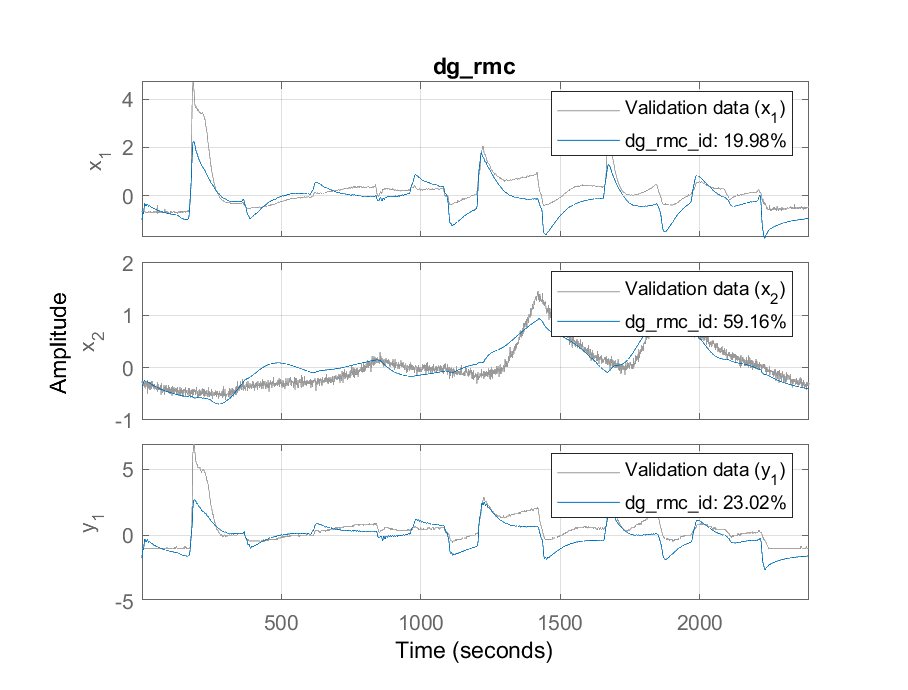
\includegraphics[width=0.7\textwidth]{Part3/figs/4_figs/dg_valid.eps}
    \caption{Comparison of the identified model with the normalized RMC test data for degreened catalyst}
    \label{fig:dg_comp}
\end{figure}

\begin{figure}[h]
    \centering
    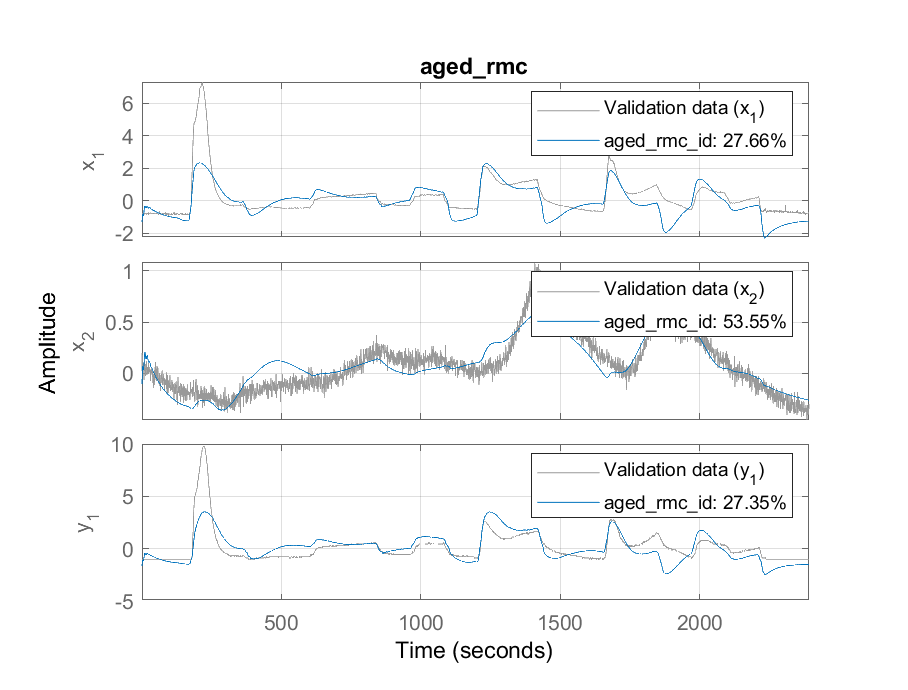
\includegraphics[width=0.7\textwidth]{Part3/figs/4_figs/aged_valid.eps}
    \caption{Comparison of the identified model with the normalized RMC test data for aged catalyst}
    \label{fig:ag_comp}
\end{figure}

Test-cell data (sampled at $5\, Hz$) from three tests (Ramped Mode Cycle (RMC),
hot and cold Federal Test Procedure (FTP))
on both aged and degreened catalysts is used for model structure validation and
model parameter estimation. The validation is done by comparing the test-cell
(experimental) response with the simulation using the estimated model
parameters (Figures~\ref{fig:dg_comp} and \ref{fig:ag_comp}). $\%fit$ is
calculated on the entire time-series of experimental data and simulation to arrive
at the goodness of fit for the model structure. This indicates the percent of
the output data that is captured by the model structure.

As shown in Table~\ref{tab:pfit}, the model structure fits reasonably well
in the cases of RMC and hot FTP data sets. The linear model structure doesn't
capture the dynamics in cold FTP case as the temperature fluctuations are
greater than $\pm 50\, ^0 C$ ($\approx \pm 100\, ^0C$) for which the linear
approximation of the rate constants (\ref{eqn::rate_approx}) is not valid.


\begin{table}[h]
\caption{Model structure validation for test data using prediction error} \label{tab:pfit}
    \begin{center}
    \begin{tabular}{| l | r l | r l |}
        \hline
 & \textbf{Aged} & \textbf{Data} & \textbf{Degreened} & \textbf{Data}
\\
\textbf{Test} & $NO_x$    & $NH_3$    &  $NO_x$   & $NH_3$   \\
& $(\%fit)$ & $(\%fit)$ &  $(\%fit)$& $(\%fit)$\\ \hline
        RMC           & $27.66$ & $53.55$ & $19.98$ & $59.16$ \\ \hline
        hot FTP       & $7.105$ & $38.31$ & $7.385$ & $56$\\ \hline
        cold FTP*      & $23.19$ & $-32.88$& $23.24$ & $-1.77$\\ \hline
\end{tabular}
    \end{center}
\itbf{Note}: $\%fit = 100 \times \lr{1 - \frac{\norm{Y- \hat Y}}{\norm{Y -
mean(Y)}}}$ is the percentage of the measured output that was explained by the
model.\\
*Cold FTP data set is not in the operating range of the linearized model.
\end{table}


The model structure can be further utilized for characterizing catalyst aging
and for diagnostic purposes. Specifically, the values of $N_{12}/\bar x$ could
be a good indicator of the catalyst aging if its value is statistically
different for aged and degreened catalysts. This value for the data sets is
tabulated in Table~\ref{tab:N12_comp}. The statistical validation of
difference in the value of $N_{12}/\bar x$ for aged and degreened catalysts is left for future work.

\begin{table}[h]
\caption{Comparison of $N_{12}/\bar x$ estimate for aged and degreened
    catalysts in test data} \label{tab:N12_comp}
    \centering
    \begin{tabular}{|l|c|c|}
        \hline
        \textbf{Test Data} & \textbf{Aged Data} & \textbf{Degreened Data}\\ \hline
        RMC                & 0.0116        & 0.0034 \\ \hline
        hot FTP            & 0.0099        & 0.0030 \\ \hline
        cold FTP           & -0.0281       & -0.0241 \\ \hline
    \end{tabular}
\end{table}

\section{Remarks}
The work showcases the effectiveness of using a linearized model dynamics of
an SCR-ASC system for diagnostics. The model, derived from first principles and
grounded on reasonable assumptions, provides a simplified yet insightful
perspective on the SCR system dynamics. This simplification facilitates the
application of system identification methods to obtain unique parameter values.
The model's validity is confirmed using experimental data from test-cell under
specific operating conditions. A particular focus is placed on input gain from
urea dosing to tail-pipe $NO_x$ ($N_{12}$), which is a monotonic function of
catalyst's nominal and total molar storage capacity, proving valuable for
monitoring catalyst aging.

% \input{Part3/4_subs/apx_secs/symbs.tex}
\section*{Appendix}
\input{Part3/4_subs/apx_secs/transfer_funcs.tex}
\input{Part3/4_subs/apx_secs/regressors.tex}
\input{Part3/4_subs/apx_secs/mdl_parm_def.tex}


\chapter{Discrete Nonlinear Model Development for Urea SCR-ASC Dynamics}

One of the fundamental assumptions in the diesel engine SCR-ASC modelling, CSTR, reverts the causality in the reaction
rate constants, when the model order is reduced by considering a single cell. The present work circumvents the problem
by discarding the CSTR assumption and modelling the time evolution of the sensor signals when a "plug" or "parcel" of
the exhaust gasses flows through the chamber.

Such a time evolution introduces constraints on the model due to sampling limitations. To capture the transient
dynamics, the sampling time should be significantly smaller than the "residence time" of the reactants inside the
SCR-ASC chamber. If that is not the case as is the situation with the present available test and truck data, time integrated states assuming zero-order holds during the transients need to be introduced into the model and the input-output model can be derived from the resulting state-space model.

The modelling approach involves following the evolution of the measurement signals at the input and the output of the
system. As the plug of fluid flows through the chamber, these measurements can be correlated based on the conservation
of moles within the fluid plug.

\section{Ammonia Adsorption/Desorption Process Dynamics}
\begin{figure}[h!]
    \centering
    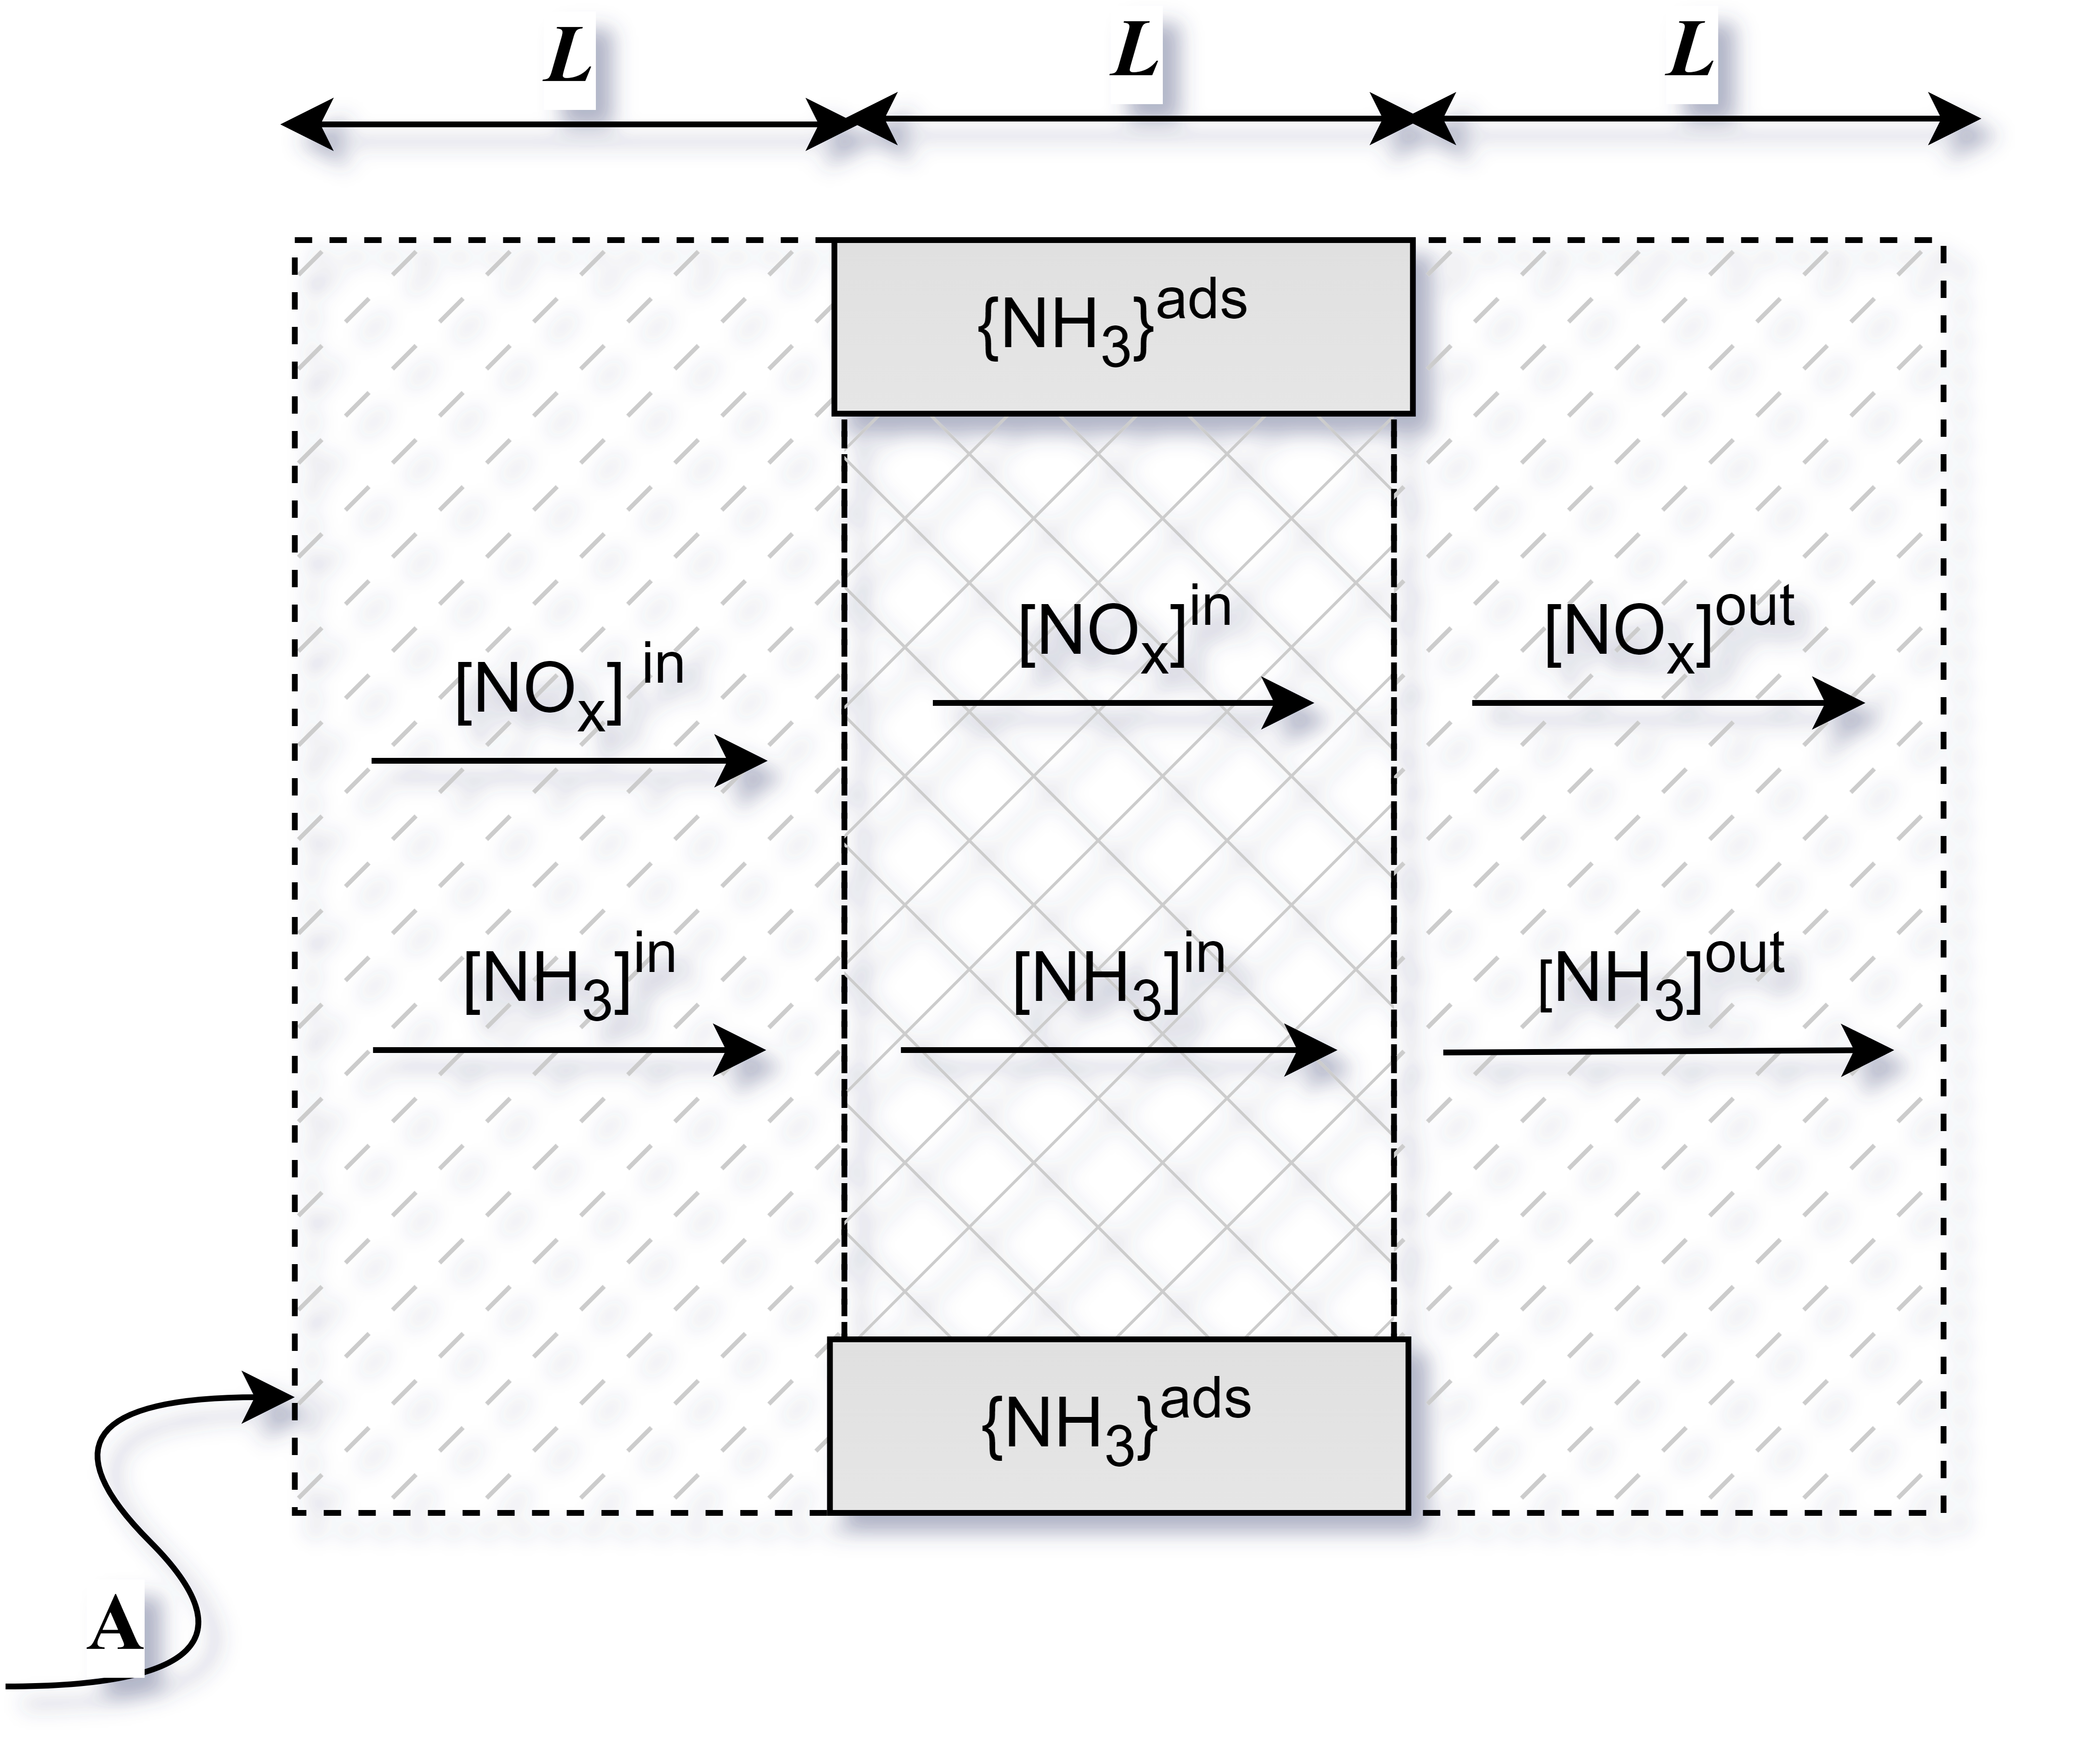
\includegraphics[width=0.5\textwidth]{Part3/figs/plug_flow_discrete.png}
    \caption{Discrete plug-flow reactor model}
    \label{fig:plug_flow_discrete}
\end{figure}
%===
The ammonia adsorption/desorption process dynamics involve all the three above-mentioned reactions. The gaseous ammonia
that enters the catalyst chamber gets adsorbed onto the free sites on the catalyst surface at a rate proportional to the
volumetric concentration of the gaseous ammonia and the surface concentration of the free sites. The adsorbed ammonia
then either reacts with the gaseous $NO_x$ (Eiley-Rideal Mechanism) releasing $N_2$ and $H_2O$ or decomposes to form
$N_2$ and $H_2O$ (Surface Decomposition). In either case, the process frees up the adsorption sites for the next cycle
of gaseous ammonia.
%===
\begin{align*}
    4 NH_3 ^{ads} + 4 NO + O_2 &\xrightarrow[]{k_{scr}} 4 N_2 + 6 H_2O \\
    4 NH_3^{ads} + 3 O_2 &\xrightarrow[]{k_{oxi}} 2 N_2 + 6 H_2O \\
    NH_3 + \Theta_{free} &\xrightleftharpoons[k_{des}]{k_{ads}} NH_3^{ads}
\end{align*}
Thus, the rate of ammonia adsorption on the catalyst surface can be modeled as:
\begin{align*}
    \frac{d \con{NH_3}^{ads}}{dt} &= r_{ads} - r_{des} - r_{scr} - r_{oxi}\\
    r_{ads} &= k_{ads} \con{NH_3}^{in} \lr{\Gamma - \con{NH_3}^{ads}} \qquad \lrb{\Gamma = \frac{\Theta_{free} - \Theta_{occupied}}{A_{scr}}}\\
    r_{des} &= k_{des} \con{NH_3}^{ads}\\
    r_{scr} &= k_{scr} \con{NH_3}^{ads} \con{NO_x}^{in}\\
    r_{oxi} &= k_{oxi} \con{NH_3}^{ads}\\
    \dot{\con{NH_3}}^{ads} &= \Gamma \underbrace{k_{ads} \con{NH_3}^{in}}_{\gamma_{ads}} - \con{NH_3}^{ads} \underbrace{\lr{k_{ads} \con{NH_3}^{in} + k_{des} + k_{scr} \con{NO_x}^{in} + k_{oxi}}}_{\gamma_{des}}
\end{align*}
\itbf{Note:} $\Gamma$ and $\con{NH_3}^{ads}$ are surface concentrations (in $moles/cm^2$) while the rest are volumetric
concentrations (in $moles/cm^3$). The rate constant units are adjusted appropriately to make the rate equations
consistent.

The units of all the rates and rate constants are tabulated below:
\begin{align*}
    r_{ads} &= \frac{moles}{cm^2 \cdot s} &
    k_{ads} &= \frac{cm^3}{moles \cdot s} \\
    r_{des} &= \frac{moles}{cm^2 \cdot s} &
    k_{des} &= s^{-1} \\
    r_{scr} &= \frac{moles}{cm^2 \cdot s} &
    k_{scr} &= \frac{cm^3}{moles \cdot s} \\
    r_{oxi} &= \frac{moles}{cm^2 \cdot s} &
    k_{oxi} &= s^{-1}
\end{align*}
%===
\itbf{Note:}In this section we are interested in the Surface rates where the products are assumed to linger just on the
surface of the catalyst. The surface rates of the gaseous products/reactants can be converted to volumetric rates by
using the conversion factor $A_{scr}/V$ where $A_{scr}$ is the area of the SCR catalyst and V is the volume of the
catalyst chamber. This assumes that there is instantaneous mixing of the close-to-surface moles with the gaseous moles.
Thus,
\begin{align}
    k^{vol} = \underbrace{\lr{\frac{A_{scr}}{V}}}_{k_{s2v} \, (cm^{-1})} k^{surf}
\end{align}
% ==============================================================================
\subsection{Molar conservation at the scale of residence time}
%===
The molar storage on the catalyst surface changes at the end of every residence time and a "fresh" set of gaseous
reactants enters the catalyst chamber. And, within the sample time, the volumetric concentrations of the gaseous
reactants can be considered constant. \itbf{Let there be $n$ residence times within one sample time.} It is implicitly
assumed that there are integer number of residence times within one sample time. When that is not the case, the
resulting is error is attributed to model structure error. Noting that $\lrf{\bullet}$ denotes moles and $\lrb{\bullet}$ denotes the concentration of the species, the molar conservation for the adsorption/desorption process can be written as:
%===
\begin{align*}
    \mol{NH_3}^{ads} (k + \tau) &= \mol{NH_3}^{ads} (k) + A_{scr} \int_{0}^{\tau} \dot{\con{NH_3}}^{ads} (k) dt\\
    \mol{NH_3}^{ads} (k + 2\tau) &= \mol{NH_3}^{ads} (k + \tau) + A_{scr} \int_{0}^{\tau} \dot{\con{NH_3}}^{ads} (k + \tau) dt\\
    \vdots&\\
    \mol{NH_3}^{ads} (k + n\tau) &= \mol{NH_3}^{ads} (k + (n-1)\tau) + A_{scr} \int_{0}^{\tau} \dot{\con{NH_3}}^{ads} (k + (n-1)\tau) dt
\end{align*}
%===
\begin{align*}
    \mol{NH_3}^{ads}(k + 1) = \mol{NH_3}^{ads} (k + n\tau) &= \mol{NH_3}^{ads} (k) + A_{scr} \sum_{i=0}^{n-1} \int_{0}^{\tau} \dot{\con{NH_3}}^{ads} (k + i\tau) dt
\end{align*}
%==
Writing the above equation in terms of surface concentrations:
\begin{align*}
    \con{NH_3}^{ads}(k + 1) = \con{NH_3}^{ads} (k + n\tau) &= \con{NH_3}^{ads} (k) + \underbrace{\sum_{i=0}^{n-1} \int_{0}^{\tau} \dot{\con{NH_3}}^{ads} (k + i\tau)}_{\Omega(k)}   dt
\end{align*}
%===
$\Omega(k)$ is the total change in the surface concentration of adsorbed ammonia
within one sample time.

% ==============================================================================
\subsection{Calculating the total surface concentration change of adsorbed ammonia within one sample time $\Omega(k)$}
%===
The volumetric concentrations of the gaseous reactants are assumed to be
constant within the sample time, while the surface concentrations change at the
end of every residence time.
\begin{align*}
    \dot{\con{NH_3}}^{ads} (k + i\tau) &= r_{ads} (k + i \tau) - r_{des} (k + i \tau) - r_{scr} (k + i \tau) - r_{oxi} (k + i \tau)\\
    %===
    r_{ads} (k + i \tau) &= k_{ads} \con{NH_3}^{in}(k) \lr{\Gamma - \con{NH_3}^{ads} (k + i \tau)}\\
    r_{des} (k + i \tau) &= k_{des} \con{NH_3}^{ads}(k + i \tau)\\
    r_{scr} (k + i \tau) &= k_{scr} \con{NH_3}^{ads}(k + i \tau) \con{NO_x}^{in}(k)\\
    r_{oxi} (k + i \tau) &= k_{oxi} \con{NH_3}^{ads}(k + i \tau)\\
    \gamma_{ads} (k) &= k_{ads} \con{NH_3}^{in}(k)\\
    \gamma_{des} (k) &= \lr{k_{ads} \con{NH_3}^{in}(k) + k_{des} + k_{scr} \con{NO_x}^{in}(k) + k_{oxi}}\\
    %===
    \dot{\con{NH_3}}^{ads} (k + i\tau) &= \Gamma \gamma_{ads} (k) - \con{NH_3}^{ads} (k + i \tau) \gamma_{des} (k)
\end{align*}

Calculating the expression for $\Omega(k)$:
\begin{align*}
    \Omega(k) &= \sum_{i=0}^{n-1} \int_{0}^{\tau} \dot{\con{NH_3}}^{ads} (k + i\tau) dt\\
    &= \sum_{i=0}^{n-1} \dot{\con{NH_3}}^{ads} (k + i\tau) \tau \qquad \lrb{\because \text{The rate is assumed to be constant within the residence time}}\\
    &= \sum_{i=0}^{n-1} \lr{\Gamma \gamma_{ads} (k) - \con{NH_3}^{ads} (k + i \tau) \gamma_{des} (k)} \tau\\
    &= \tau n \Gamma \gamma_{ads} (k) - \tau \gamma_{des} (k) \underbrace{\sum_{i=0}^{n-1} \con{NH_3}^{ads} (k + i \tau) }_{n \sigma(k)} \\
    &= n \tau \lr{\Gamma \gamma_{ads} (k) - \sigma(k) \gamma_{des} (k)}
\end{align*}

The term $\sigma(k)$ is unknown and unobservable. It is the average surface
concentration at the end of every residence time within the sample time.

Moreover, we can get the expression for average rate of change of the surface
concentrations within the sample time as:
\begin{align*}
    \dot{\con{NH_3}}^{ads} (k) &= \frac{\Omega(k)}{\tau n} = \Gamma \gamma_{ads} (k) - \sigma(k) \gamma_{des} (k)\\
    &= \Gamma k_{ads} \con{NH_3}^{in}(k) - \sigma(k) \lr{k_{ads} \con{NH_3}^{in}(k) + k_{des} + k_{scr} \con{NO_x}^{in}(k) + k_{oxi}}
\end{align*}

% ==============================================================================
\subsection{Ammonia adsorption/desorption process dynamics model}
Substituting the expression for $\Omega(k)$ in the equation for
$\con{NH_3}^{ads}(k + 1)$:
%===
\begin{align*}
    \con{NH_3}^{ads}(k + 1) &= \con{NH_3}^{ads} (k) + n \tau \lr{\Gamma \gamma_{ads} (k) - \sigma(k) \gamma_{des} (k)}\\
    &= \con{NH_3}^{ads}(k) + n \tau \Gamma k_{ads} \con{NH_3}^{in}(k) \\
    &\quad - n \tau \sigma(k) \lr{k_{ads} \con{NH_3}^{in}(k) + k_{des} + k_{scr} \con{NO_x}^{in}(k) + k_{oxi}}
\end{align*}
%===
\input{Part3/5_subs/4_subs/sig_approx.tex}

\section{$NO_x$ Process Dynamics}

The $NO_x$ process dynamics involve only the selective catalytic reduction reaction. The gaseous $NO_x$ that enters the
catalyst chamber reacts with the adsorbed ammonia on the surface and forms $N_2$ and $H_2O$ (Eiley-Rideal Mechanism).
The process frees up the adsorption sites for the next cycle of gaseous ammonia. The reaction rate is proportional to
the volumetric concentration of the gaseous $NO_x$ and the surface concentration of the adsorbed ammonia.
\begin{align}
    4 NH_3 ^{ads} + 4 NO + O_2 &\xrightarrow[]{k_{scr}} 4 N_2 + 6 H_2O
\end{align}

Thus, the rate of $NO_x$ reduction on the catalyst surface can be modeled as:
\begin{align}
    \frac{d \con{NO_x}^{scr}}{dt} &= - k_{s2v} r_{scr} \\
    r_{scr} &= k_{scr} \con{NH_3}^{ads} \con{NO_x}^{in}\\
    \dot{\con{NO_x}}^{scr} &= -k_{s2v} k_{scr} \con{NH_3}^{ads} \con{NO_x}^{in}
\end{align}

% ==============================================================================
\subsection{Molar conservation at the scale of residence time}

Similar to the ammonia adsorption/desorption process, at the end of every residence time, a fresh parcel of gaseous
reactants enters the catalyst chamber. Thus, the molar conservation for the $NO_x$ reduction process can be
correlated with the inlet and outlet molar concentrations of the $NO_x$ at the beginning and the end of residence time. Thus,
\begin{align*}
    \mol{NO_x}^{out} (k + \tau) &= \mol{NO_x}^{in} (k) + V \int_{0}^{\tau}  \dot{\con{NO_x}}^{scr} (k) dt\\
    \mol{NO_x}^{out} (k + 2\tau) &= \mol{NO_x}^{in} (k + \tau) + V \int_{0}^{\tau} \dot{\con{NO_x}}^{scr} (k+\tau)  dt\\
    \vdots &\\
    \mol{NO_x}^{out} (k + n\tau) &= \mol{NO_x}^{in} (k + (n-1)\tau) + V \int_{0}^{\tau} \dot{\con{NO_x}}^{scr} (k+(n-1)\tau) dt
\end{align*}

The above equations show that the measurement of $NO_x$ concentration at the outlet depends only on the measurement of
the $NO_x$ concentration at the inlet one residence time before. Thus, there is no integrating effect of the $NO_x$
within the sample time. Writing in terms of volumetric concentrations, we have:

\begin{align*}
    \con{NO_x}^{out} (k + n\tau) &= \con{NO_x}^{in} (k + (n-1)\tau) + \int_{0}^{\tau}  \dot{\con{NO_x}}^{scr} (k + (n-1)\tau) dt
\end{align*}

Introducing the following two approximations:
\begin{enumerate}
    \item Zero-order-hold for the inlet concentration of $NO_x$:
        \begin{align*}
            \con{NO_x}^{in} (k + i \tau) &\approx \con{NO_x}^{in} (k) \qquad \forall i < n
        \end{align*}
    \item Using average surface concentration at the sample for the surface concentration of the adsorbed ammonia:
        \begin{align*}
            \con{NH_3}^{ads} (k + i \tau) &\approx \sigma(k) \qquad \forall i < n
        \end{align*}
\end{enumerate}

Thus,
\begin{align*}
    \dot{\con{NO_x}}^{scr} (k + i \tau) =  \dot{\con{NO_x}}^{scr} (k) = -k_{s2v} k_{scr} \sigma(k) \con{NO_x}^{in} (k) \qquad \forall i < n
\end{align*}


Thus, we have the following expression for the $NO_x$ process dynamics:

\begin{align*}
    \con{NO_x}^{out} (k + n\tau) &= \con{NO_x}^{in} (k) - k_{s2v} k_{scr} \sigma(k) \con{NO_x}^{in} (k) \tau\\
    \implies \con{NO_x}^{out} (k + 1) &= \con{NO_x}^{in} (k) \lr{1 - k_{s2v} k_{scr} \sigma(k) \tau}
\end{align*}


% ==============================================================================

\newpage
\section{Gaseous Ammonia Process Dynamics}
The gaseous ammonia process dynamics involve the adsorption and desorption dynamics. The gaseous ammonia that enters the
catalyst chamber gets adsorbed on the free sites on the catalyst surface at a rate proportional to the volumetric
concentration of the gaseous ammonia and the surface concentration of the free sites. A part of adsorbed ammonia then
desorbs back to the gas phase at a rate that is proportional to the surface concentrations of the adsorbed ammonia.
\begin{align*}
    NH_3 + \Theta_{free} &\xrightleftharpoons[k_{des}]{k_{ads}} NH_3^{ads}
\end{align*}

Thus, the rate of change of gaseous $NH_3$ on the catalyst surface can be modeled as:
\begin{align*}
    \frac{d \con{NH_3}^{scr}}{dt} &= k_{s2v} (-r_{ads} + r_{des}) \\
    r_{ads} &= k_{ads} \con{NH_3}^{in} \lr{\Gamma - \con{NH_3}^{ads}}\\
    r_{des} &= k_{des} \con{NH_3}^{ads}\\
    \dot{\con{NH_3}}^{scr} &= -k_{s2v}k_{ads} \con{NH_3}^{in} \lr{\Gamma - \con{NH_3}^{ads}} + k_{s2v} k_{des} \con{NH_3}^{ads}\\
\end{align*}

% ==============================================================================
\subsection{Molar conservation at the scale of residence time}

Similar to the ammonia adsorption/desorption process, at the end of every residence time, a fresh parcel of gaseous
reactants enters the catalyst chamber. Thus, the molar conservation for the gaseous $NH_3$ adsorption/desorption process
can be correlated with the inlet and outlet molar concentrations of the $NH_3$ at the beginning and the end of residence
time. Similar to the $NO_x$ process dynamics the measurement of $NH_3$ concentration at the outlet depends only on the
measurement of the $NH_3$ concentration at the inlet one residence time before. That is, there is no integrating effect
of the $NH_3$ within the sample time either. Writing in terms of volumetric concentrations, we have:

\begin{align*}
    \con{NH_3}^{out} (k + n\tau) &= \con{NH_3}^{in} (k + (n-1)\tau) + \int_{0}^{\tau}  \dot{\con{NH_3}}^{scr} (k + (n-1)\tau) dt
\end{align*}

Introducing the following two approximations:
\begin{enumerate}
    \item Zero-order-hold for the inlet concentration of $NH_3$:
        \begin{align*}
            \con{NH_3}^{in} (k + i \tau) &\approx \con{NH_3}^{in} (k) \qquad \forall i < n
        \end{align*}
    \item Using average surface concentration at the sample for the surface concentration of the adsorbed ammonia:
        \begin{align*}
            \con{NH_3}^{ads} (k + i \tau) &\approx \sigma(k) \qquad \forall i < n
        \end{align*}
\end{enumerate}

Thus,
\begin{align*}
    \dot{\con{NH_3}}^{scr} (k + i \tau) &= -k_{s2v}k_{ads} \con{NH_3}^{in} \lr{\Gamma - \sigma(k)} + k_{s2v} k_{des} \sigma(k)
    \qquad \forall i < n
\end{align*}


Thus, we have the following expression for the $NH_3$ process dynamics:

\begin{align*}
    \con{NH_3}^{out} (k + n\tau) &= \con{NH_3}^{in} (k) - \tau k_{s2v}k_{ads} \con{NH_3}^{in}(k) \lr{\Gamma - \sigma(k)} + \tau k_{s2v} k_{des} \sigma(k)\\
    \con{NH_3}^{out} (k + 1) &= \con{NH_3}^{in}(k) \lr{1 - \tau k_{s2v}k_{ads} \lr{\Gamma - \sigma(k)}} + \tau k_{s2v} k_{des} \sigma(k)
\end{align*}

\newpage
\section{Urea Dosing Process Dynamics}
The urea dosing dynamics involve the following reactions:
\begin{align*}
    NH_2 - CO - NH_2 (liquid) &\longrightarrow NH_2 - CO - NH_2^* + x H_2 O
                & &[\text{AdBlue evaporation}] \\
    NH_2 - CO - NH_2^*  &\longrightarrow  HNCO + NH_3
                & &[\text{Urea decomposition}] \\
    HNCO + H_2O &\longrightarrow NH_3 + CO_2
                & &[\text{Isocynic acid hydrolysis}] \\
\end{align*}

The above reactions can be aggregated into:
\begin{align*}
    NH_2 - CO - NH_2 (liquid) &\longrightarrow 2 NH_3 + CO_2 + x H_2 O
\end{align*}

The rate of ammonia production is twice the rate of decomposition of the urea in the solution (AdBlue). Thus,
\begin{align*}
    \frac{d \con{NH_3}^{in}}{dt} &= 2 r_{u}\\
    r_{u} &= k_{u} \con{NH_2 - CO - NH_2} \qquad (constant)
\end{align*}

As the concentration of urea in the solution is constant, the above rate becomes a constant. Thus, the total moles of
ammonia produced at the inlet within a residence time would be:
\begin{align*}
    \mol{NH_3}^{in} (k) &= \tau \times \underbrace{2 r_{u}}_{\text{Rate of decomposition}} \times \underbrace{\tau u_{inj} (k)}_{\text{Volume injected}}
\end{align*}
Where $u_{inj}$ urea-solution injection rate in $ml/s$.

Thus, we have the inlet volumetric concentration of ammonia as:
\begin{align*}
    \con{NH_3}^{in} (k) &= \frac{\mol{NH_3}^{in} (k)}{V}
                          = \frac{2 r_u}{V} \times \tau^2 \times u_{inj} (k)
\end{align*}

Substituting, $\tau = \frac{V \rho_0}{F}$, we get:
\begin{align}
    \con{NH_3}^{in} (k) &= 2r_u V \rho^2_0 \times \frac{u_{inj}(k)}{F^2}
\end{align}


The above reciprocal relationship breaks down at zero flow rate which makes sense physically. Within the operating conditions we have:

% \begin{align*}
%     \delta  \con{NH_3}^{in} (k) &= -4r_u V \times \frac{\bar u_{inj}}{\bar{f}_v^3} \delta f_v
%                                    + 2r_u V \times \frac{\delta u_{inj}}{\bar f_v^2}\\
% \end{align*}
%
% The linearized approximation model would be:
%
% \begin{align*}
%     \con{NH_3}^{in}(k) &= \con{NH_3}^{in}_0 + \delta \con{NH_3}^{in} (k)\\
%                        &= 2r_u V \times \frac{\bar u_{inj}}{ \bar f_v^2}
%                          + 2r_u V \times \frac{\delta u_{inj}}{\bar f_v^2}
%                          -4r_u V \times \frac{\bar u_{inj}}{\bar{f}_v^3} \delta f_v\\
%                        &= 2r_u V \times \frac{u_{inj}(k)}{ \bar f_v^2}
%                          -4r_u V \times \frac{\bar u_{inj}}{\bar{f}_v^3} \delta f_v(k)
%                          \qquad \lrb{\because \bar u_{inj} + \delta u_{inj} = u_{inj}}
% \end{align*}
% Introducing the $\delta f_v$ as function of $F$ and $T$ from equation \ref{eqn::fv_approx},
% \begin{align*}
%     \con{NH_3}^{in}(k) &= \lr{\frac{2r_u V}{\bar f_v^2}} u_{inj}(k)
%                           -\lr{\frac{ 4r_u V \bar u_{inj}}{\bar{f}_v^3}}\lr{\frac{1}{\mu} \lr{F_0 \delta T + T_0 \delta F} } \\
%                        &= \lr{\frac{2r_u V}{\bar f_v^2}} u_{inj}(k)
%                           -\lr{\frac{ 4r_u V \bar u_{inj} F_0 }{\mu \bar{f}_v^3}} \delta T
%                           -\lr{\frac{ 4r_u V \bar u_{inj} T_0 }{\mu \bar{f}_v^3}} \delta F
% \end{align*}
% Dropping the $\delta$ for notational convenience,
\begin{align}
    \con{NH_3}^{in}(k) &= \nu_u \frac{u_{inj}}{F^2}    \label{eqn::urea_inj}
\end{align}
where,
\begin{align*}
    \nu_u &= 2r_u V \rho^2_0\\
    T_{min} &\leq T \leq T_{max}\\
    F_{min} &\leq F \leq F_{max}
\end{align*}

\section{Linear Parameter Model for SCR Process Dynamics with Urea Dosing \label{sec::proc_dyn}}
From previous derivations, we have the complete process dynamics of SCR-ASC dynamics with urea dosing as:

\begin{enumerate}
    \item Urea dosing dynamics:
    \begin{align*}
    \con{NH_3}^{in} (k) &= 2r_u V \times \frac{u_{inj}(k)}{f_v^2}
    \end{align*}

    \item $NO_x$ reduction dynamics:
    \begin{align*}
    \con{NO_x}^{out} (k + 1) &= \con{NO_x}^{in} (k) \lr{1 - k_{s2v} k_{scr} \sigma(k) \tau}
    \end{align*}

    \item Gaseous ammonia dynamics:
    \begin{align*}
    \con{NH_3}^{out} (k + 1) &= \con{NH_3}^{in}(k) \lr{1 - \tau k_{s2v}k_{ads} \lr{\Gamma - \sigma(k)}} + \tau k_{s2v} k_{des} \sigma(k)
    \end{align*}

    \item Ammonia adsorption/desorption dynamics:
 \begin{align*}
        \sigma(k + 1) &= \sigma(k)
        + n\tau k_{ads} \con{NH_3}^{in} \lr{\Gamma - \sigma(k)}
        - n \tau \lr{k_{oxi} + k_{des}} \sigma(k)
        - n \tau k_{scr} \con{NO_x}^{in}(k) \sigma(k)
    \end{align*}
\end{enumerate}

The above four equations are the complete process dynamics of SCR-ASC dynamics with urea dosing. The above equations are
nonlinear and coupled with implicit dependence on temperature and flow rate. In this section the above equations are
rewritten in a parametric form with standard state-space representation. For convenience and clarity '(k)' is dropped
from the variables.


Further, the models that have reciprocals and expoenetials of inputs are linearized about the operating points. These include:
\begin{enumerate}
    \item Rate constants
        \begin{align}
            k_i &= m_i T + c_i
        \end{align}
    \item Residence time (\ref{eqn::res_time})
        \begin{align}
            \tau &= \frac{V \rho_0}{F} = \frac{\tau_0}{F}
        \end{align}
\end{enumerate}

The following states and inputs are defined for the system:

\begin{align*}
    x_1 &= \con{NO_x}^{out} & u_1 &= \con{NO_x}^{in} \\
    x_2 &= \con{NH_3}^{out} & u_2 &= u_{inj} \\
    x_3 &= \sigma & u_3 &= T\\
        &         & u_4 &= F
\end{align*}

Thus, linear-parameter representation of each of the processes are as follows:
%%======================================================================================================================
\input{Part3/5_subs/9_subs/urea_dosing.tex}
\input{Part3/5_subs/9_subs/general_simplification.tex}
\input{Part3/5_subs/9_subs/nox_proc.tex}
\input{Part3/5_subs/9_subs/nh3_gas.tex}
\input{Part3/5_subs/9_subs/nh3_ads.tex}
\input{Part3/5_subs/9_subs/remarks.tex}
%%======================================================================================================================







%%%%%%%%%%%%%%%%%
%% Old Stuff %%%%
%%%%%%%%%%%%%%%%%

\section{Nonlinear recursive model with linear parameters for tailpipe $NO_x$ $\lr{\con{NO_x}^{out}}$ dynamics}
Rewriting equation \ref{eqn::nox_regression} to get the adsorbed ammonia:
\begin{align*}
        x_3(k) \lrf{\pmb \phi_1^T(k) \pmb \theta_1} &= {x_1(k+1) - u_1(k)}\\
        \implies x_3(k+1) \lrf{\pmb \phi_1^T(k+1) \pmb \theta_1} &= {x_1(k+2) - u_1(k+1)}
\end{align*}
Consider \ref{eqn::nh3_ads_regression}:
\begin{align*}
     x_3(k+1) &= x_3 \pmb \phi_3^T \pmb \theta_3 + \pmb \phi_{\tau, ur} \pmb \theta_\Gamma\\
     \implies \lrf{\pmb \phi_1^T(k) \pmb \theta_1} x_3(k+1) &= \lrf{\pmb \phi_1^T(k) \pmb \theta_1} \lrf{x_3 \pmb \phi_3^T \pmb \theta_3 + \pmb \phi_{\tau, ur} \pmb \theta_\Gamma}\\
     &= \lrf{\lr{\pmb \phi_1^T(k) \pmb \theta_1}x_3(k)} \lrf{\pmb \phi_3^T \pmb \theta_3}
     + \lrf{\pmb \phi_1^T(k) \pmb \theta_1} \lrf{\pmb \phi_{\tau, ur} \pmb \theta_\Gamma}\\
     &= \lrf{{x_1(k+1) - u_1(k)}} \lrf{\pmb \phi_3^T \pmb \theta_3}
     + \lrf{\pmb \phi_1^T(k) \pmb \theta_1} \lrf{\pmb \phi_{\tau, ur} \pmb \theta_\Gamma}  \qquad \lrb{\because \ref{eqn::nox_regression}}
\end{align*}
\begin{align}
        \lrf{\pmb \phi_1^T(k) \pmb \theta_1} x_3(k+1)
        &= \lrf{{x_1(k+1) - u_1(k)}} \lrf{\pmb \phi_3^T \pmb \theta_3} + \lrf{\pmb \phi_1^T(k) \pmb \theta_1} \lrf{\pmb \phi_{\tau, ur} \pmb \theta_\Gamma}
        \label{eqn::r_nox_1}
\end{align}
Let,
\begin{align}
        f_{\phi_1}(k+1) &= \pmb \phi_1(k+1)^T \lrb{\pmb \phi_1(k) \pmb \phi_1^T(k)}^{-1} \pmb \phi_1(k)
        \label{eqn::f_phi_1}
\end{align}
Thus,
\begin{align}
        f_{\phi_1}(k+1) \lrf{\pmb \phi_1^T(k) \pmb \theta_1} &= \pmb \phi_1(k+1)^T \lrb{\pmb \phi_1(k) \pmb \phi_1^T(k)}^{-1} \pmb \phi_1(k) \lrf{\pmb \phi_1^T(k) \pmb \theta_1}
        = \pmb \phi_1^T(k+1) \pmb \theta_1
        \label{eqn::f_phi_prop}
\end{align}
Note that $f_{\phi_1}$ is a scalar. Multiplying $f_{\phi_1}(k+1)$ on both sides of equation (\ref{eqn::r_nox_1}):
\begin{align*}
      &f_{\phi_1}(k+1) \lrf{\pmb \phi_1^T(k) \pmb \theta_1} x_3(k+1)
                = \lrf{{x_1(k+1) - u_1(k)}} f_{\phi_1}(k+1)\lrf{\pmb \phi_3^T (k) \pmb \theta_3}
                + f_{\phi_1}(k+1)\lrf{\pmb \phi_1^T(k) \pmb \theta_1} \lrf{\pmb \phi^T_{\tau, ur}(k) \pmb \theta_\Gamma}\\
      %===
      &\implies {x_1(k+2) - u_1(k+1)} = \lrf{{x_1(k+1) - u_1(k)}} f_{\phi_1}(k+1)\lrf{\pmb \phi_3^T (k) \pmb \theta_3}
                + \lrf{ \lr{\pmb \phi_1^T(k+1) \pmb \theta_1} \kron \lr{\pmb \phi^T_{\tau, ur}(k) \pmb \theta_\Gamma}}
        \quad \lrb{\because \ref{eqn::f_phi_prop}}
\end{align*}
Writing in one time step ahead form:
\begin{align}
        x_1(k+1) &=  u_1(k)  +
                     \lrf{{x_1(k) - u_1(k-1)}} f_{\phi_1}(k)\lrf{\pmb \phi_3^T (k-1) \pmb \theta_3}+
                     \lrf{ \lr{\pmb \phi_1^T(k) \pmb \theta_1} \kron \lr{\pmb \phi^T_{\tau, ur}(k-1) \pmb \theta_\Gamma}}
        \label{eqn::r_nox_2}
\end{align}
%===
Expanding the terms and defining the following new regressor and parameter vectors,
\begin{align*}
        \text{Let, } \qquad &\\
        &\pmb \theta_3 = \bm{1 &
                             n \pmb \theta_{ads, ur}    &
                             n \pmb \theta_{od}         &
                             n \pmb \theta_{scr}}^T
                        = \bm{1 & \pmb \theta_{f1}}^T\\
        %==
        \text{and, } \qquad &\\
        &\because \pmb \phi_3^T(k-1) = \bm{1&
                                                  - \pmb \phi_{\tau, ur} (k-1)&
                                                  - \pmb \phi_\tau (k-1) &
                                                  - u_1(k-1) \pmb \phi_{\tau}(k-1) }\\
        %===
        &\lrf{{x_1(k) - u_1(k-1)}} f_{\phi_1}(k) \pmb \phi_3^T (k-1)  = \lrf{{x_1(k) - u_1(k-1)}} f_{\phi_1}(k) - \pmb \phi_{f1}\\
        %===
        \text{Where, } \qquad &\\
        &\pmb \phi_{f1}(k)
                = \lrf{{x_1(k) - u_1(k-1)}} f_{\phi_1}(k)
                \bm{\pmb \phi_{\tau, ur} (k-1)&
                    \pmb \phi_\tau (k-1) &
                    u_1(k-1) \pmb \phi_{\tau}(k-1) }\\
        \text{and, } \qquad &\\
        &\pmb \theta_{f1}^T = n \bm{ \pmb \theta_{ads, ur}  & \pmb \theta_{od}  & \pmb \theta_{scr}}\\
\end{align*}
We have the following properties of Kronecker product:
        \begin{align*}
                \lr{A \kron B}^T &= A^T \kron B^T \\
                \lr{A \kron B} \lr{C \kron D} &= \lr{AC} \kron \lr{BD}
        \end{align*}
Thus, Kronecker product can be rewritten into product of regressor and parameter vectors as:
\begin{align*}
        \lrf{\pmb \phi_1^T(k) \pmb \theta_1} \kron \lrf{\pmb \phi^T_{\tau, ur}(k-1) \pmb \theta_\Gamma} &=
             \lrf{ \pmb \phi_1^T(k) \kron \pmb \phi^T_{\tau, ur}(k-1) }
             \lrf{\pmb \theta_1 \kron \pmb \theta_\Gamma}\\
        \pmb \phi_{\Gamma 1} (k) &= \lrf{ \pmb \phi_1^T(k) \kron \pmb \phi^T_{\tau, ur}(k-1) } \\
        \pmb \theta_{\Gamma 1} &= \lrf{\pmb \theta_1 \kron \pmb \theta_\Gamma}
\end{align*}
The regressors coming from  of Kronecker products are will have full rank they involve the product of inputs at different time steps. Thus, they can be algorithmically computed and need not be simplified to a vector expression.

Substituting the above definitions into equation (\ref{eqn::r_nox_2}):
\begin{align}
         x_1(k+1) &=  u_1(k)  + \lrf{{x_1(k) - u_1(k-1)}} f_{\phi_1}(k) -
                     \pmb \phi_{f1}^T(k) \pmb \theta_{f1} +
                     \pmb \phi_{\Gamma 1}^T(k) \pmb \theta_{\Gamma 1}
        \label{eqn::r_nox_3}
\end{align}
Let,
\begin{align}
        \pmb \phi_{NO_x} &= \bm{-\pmb \phi_{f1} & \pmb \phi_{\Gamma 1}}\\
        \pmb \theta_{NO_x} &= \bm{\pmb \theta_{f1} & \pmb \theta_{\Gamma 1}}
\end{align}
\begin{align}
          x_1(k+1) &=  u_1(k)  + \lrf{{x_1(k) - u_1(k-1)}} f_{\phi_1}(k) +
                     \pmb \phi_{NO_x}^T (k) \pmb \theta_{NO_x}
        \label{eqn::r_nox_regression}
\end{align}

%%===
\input{Part3/5_subs/10_subs/theta_parm.tex}
\input{Part3/5_subs/10_subs/phi_alg.tex}

\graphicspath{{Part3}}
\section{Cross validation results}

\subsection{Degreened Test Data}

\begin{figure}[H]
        \begin{minipage}{0.3\textwidth}
                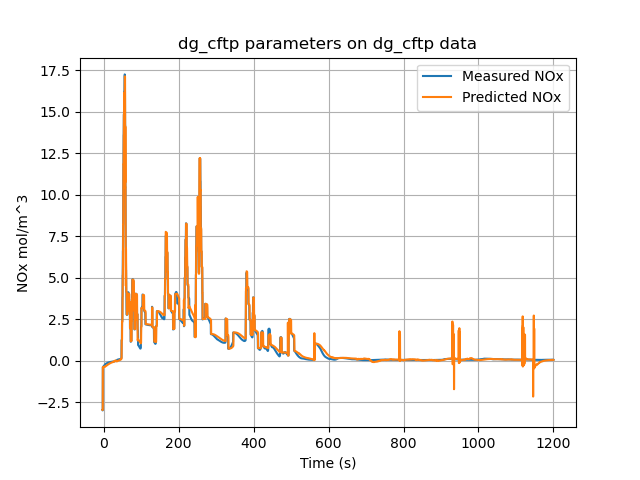
\includegraphics[width = \textwidth]{./figs/figs_new_mdl/dg_cftp_dg_cftp.png}
        \end{minipage}
        \begin{minipage}{0.3\textwidth}
                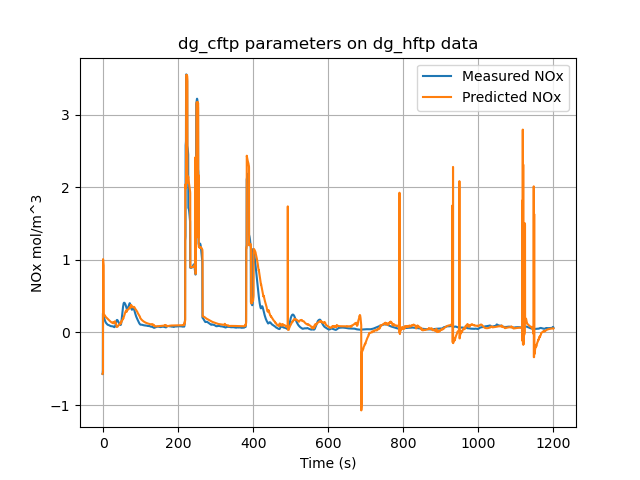
\includegraphics[width = \textwidth]{./figs/figs_new_mdl/dg_cftp_dg_hftp.png}
        \end{minipage}
        \begin{minipage}{0.3\textwidth}
                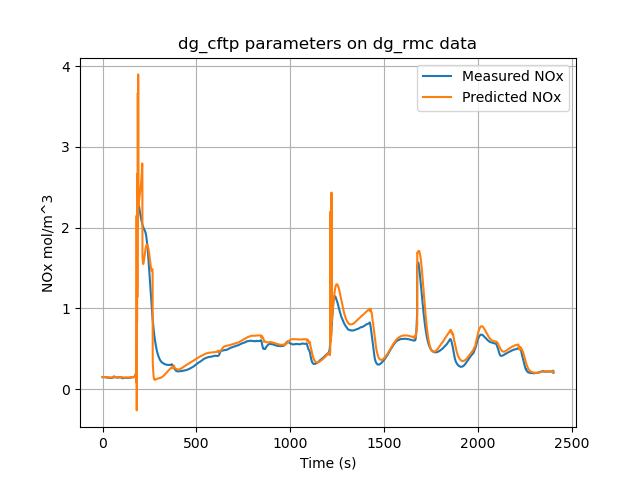
\includegraphics[width = \textwidth]{./figs/figs_new_mdl/dg_cftp_dg_rmc.png}
        \end{minipage}
        \caption{Cross validation using dg$\_$cftp parameter estimates}
\end{figure}

\begin{figure}[H]
        \begin{minipage}{0.3\textwidth}
                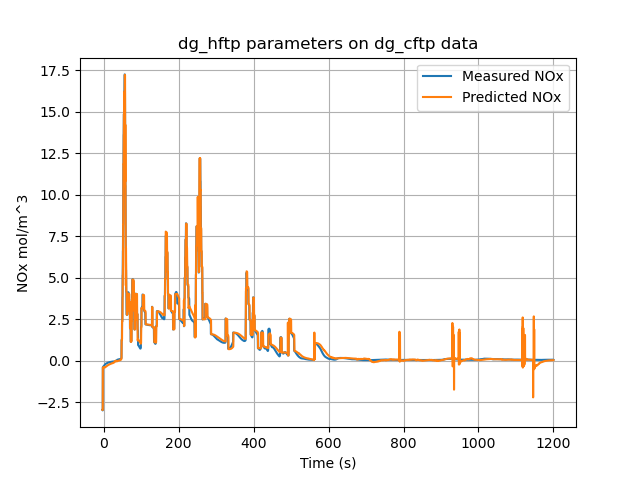
\includegraphics[width = \textwidth]{./figs/figs_new_mdl/dg_hftp_dg_cftp.png}
        \end{minipage}
        \begin{minipage}{0.3\textwidth}
                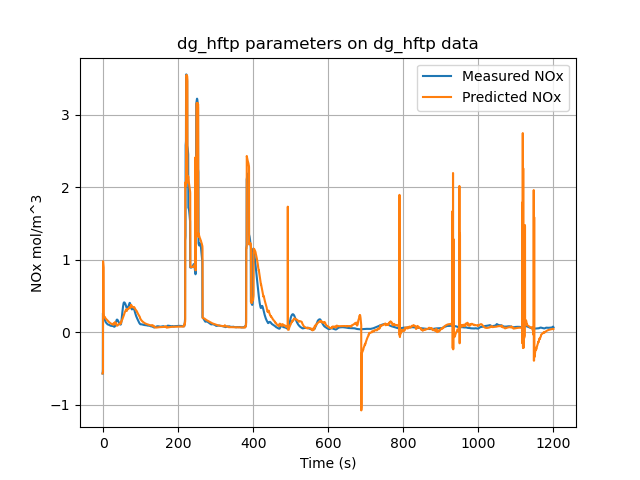
\includegraphics[width = \textwidth]{./figs/figs_new_mdl/dg_hftp_dg_hftp.png}
        \end{minipage}
        \begin{minipage}{0.3\textwidth}
                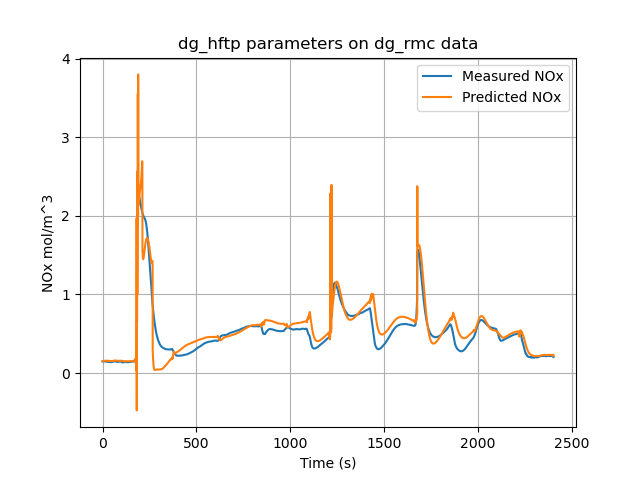
\includegraphics[width = \textwidth]{./figs/figs_new_mdl/dg_hftp_dg_rmc.png}
        \end{minipage}
        \caption{Cross validation using dg$\_$hftp parameter estimates}
\end{figure}

\begin{figure}[H]
        \begin{minipage}{0.3\textwidth}
                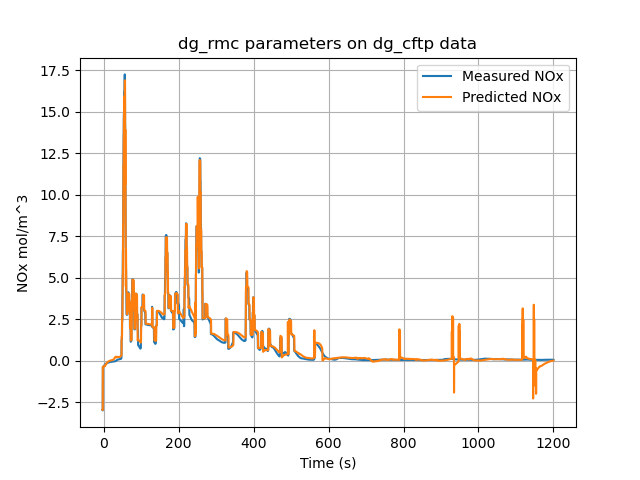
\includegraphics[width = \textwidth]{./figs/figs_new_mdl/dg_rmc_dg_cftp.png}
        \end{minipage}
        \begin{minipage}{0.3\textwidth}
                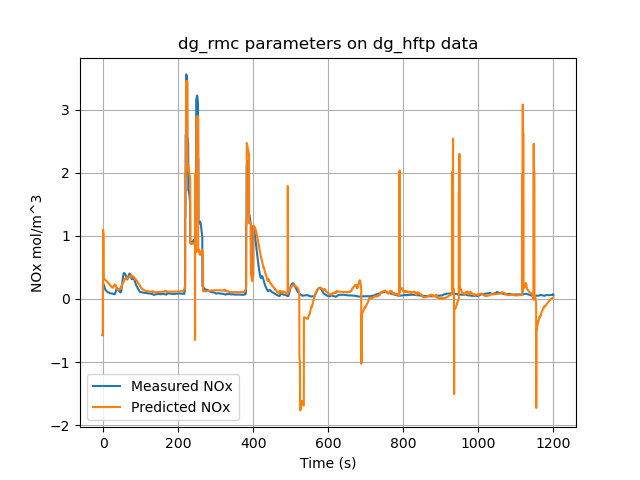
\includegraphics[width = \textwidth]{./figs/figs_new_mdl/dg_rmc_dg_hftp.png}
        \end{minipage}
        \begin{minipage}{0.3\textwidth}
                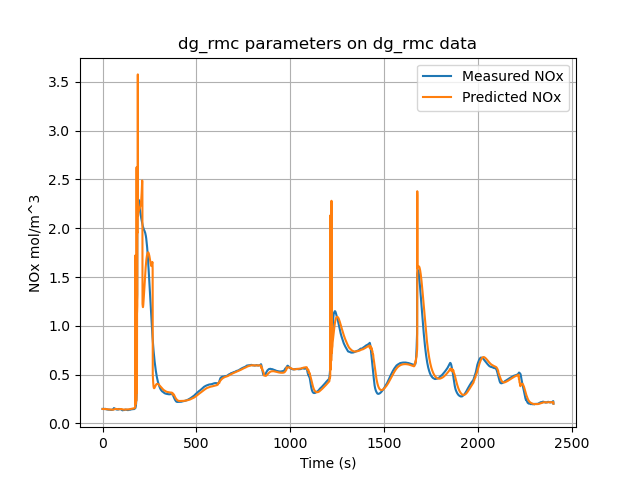
\includegraphics[width = \textwidth]{./figs/figs_new_mdl/dg_rmc_dg_rmc.png}
        \end{minipage}
        \caption{Cross validation using dg$\_$rmc parameter estimates}
\end{figure}


\subsection{Aged Test Data}

\begin{figure}[H]
        \begin{minipage}{0.3\textwidth}
                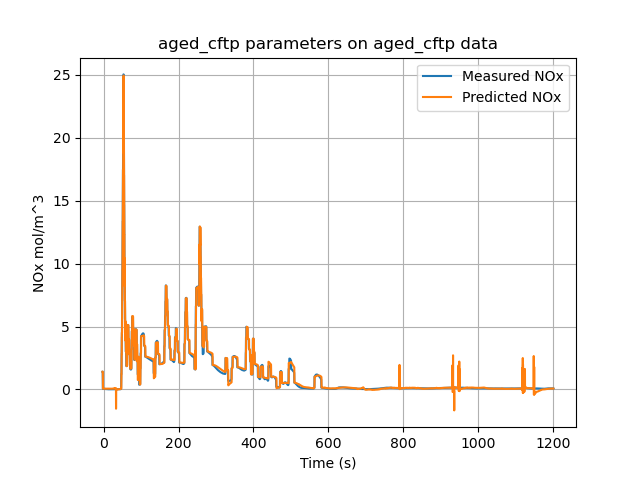
\includegraphics[width = \textwidth]{./figs/figs_new_mdl/aged_cftp_aged_cftp.png}
        \end{minipage}
        \begin{minipage}{0.3\textwidth}
                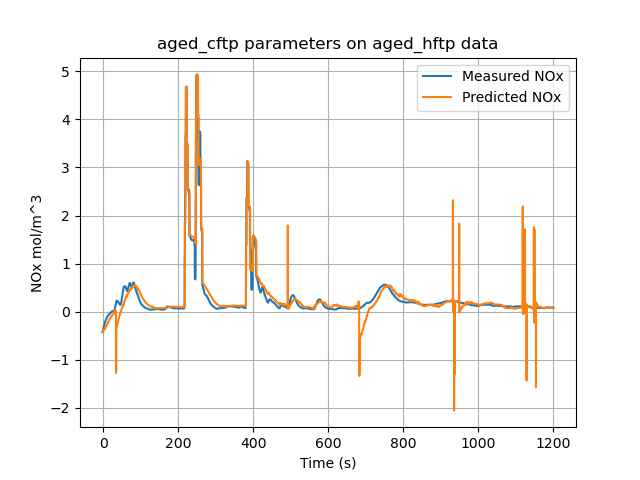
\includegraphics[width = \textwidth]{./figs/figs_new_mdl/aged_cftp_aged_hftp.png}
        \end{minipage}
        \begin{minipage}{0.3\textwidth}
                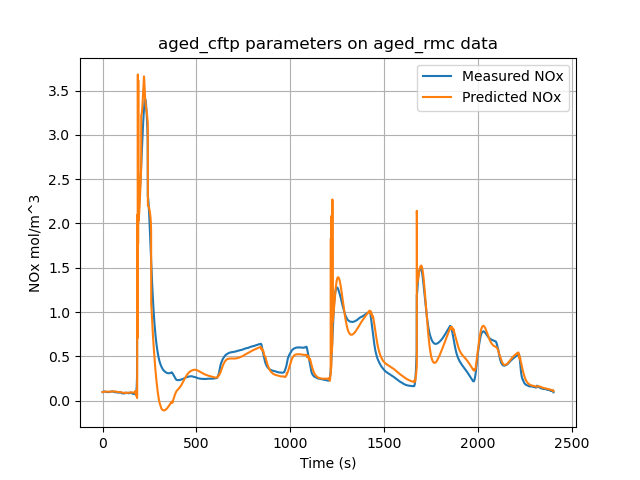
\includegraphics[width = \textwidth]{./figs/figs_new_mdl/aged_cftp_aged_rmc.png}
        \end{minipage}
        \caption{Cross validation using aged$\_$cftp parameter estimates}
\end{figure}

\begin{figure}[H]
        \begin{minipage}{0.3\textwidth}
                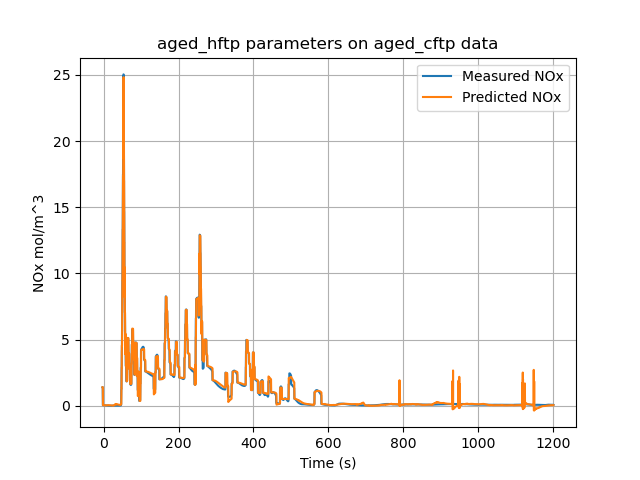
\includegraphics[width = \textwidth]{./figs/figs_new_mdl/aged_hftp_aged_cftp.png}
        \end{minipage}
        \begin{minipage}{0.3\textwidth}
                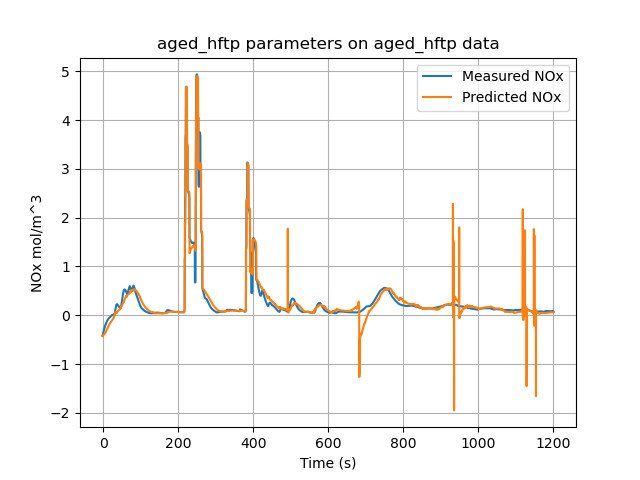
\includegraphics[width = \textwidth]{./figs/figs_new_mdl/aged_hftp_aged_hftp.png}
        \end{minipage}
        \begin{minipage}{0.3\textwidth}
                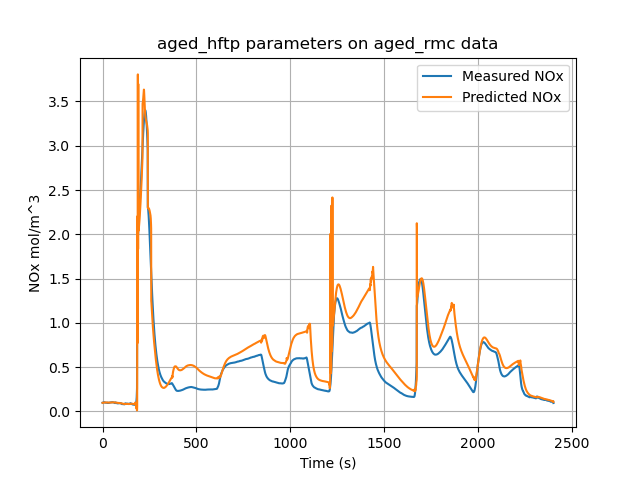
\includegraphics[width = \textwidth]{./figs/figs_new_mdl/aged_hftp_aged_rmc.png}
        \end{minipage}
        \caption{Cross validation using aged$\_$hftp parameter estimates}
\end{figure}

\begin{figure}[H]
        \begin{minipage}{0.3\textwidth}
                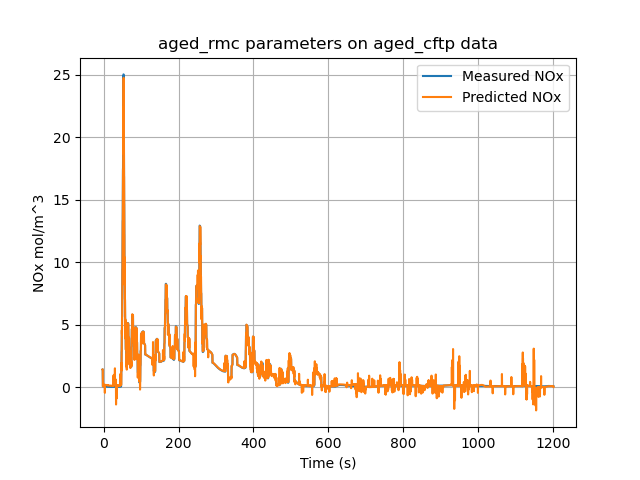
\includegraphics[width = \textwidth]{./figs/figs_new_mdl/aged_rmc_aged_cftp.png}
        \end{minipage}
        \begin{minipage}{0.3\textwidth}
                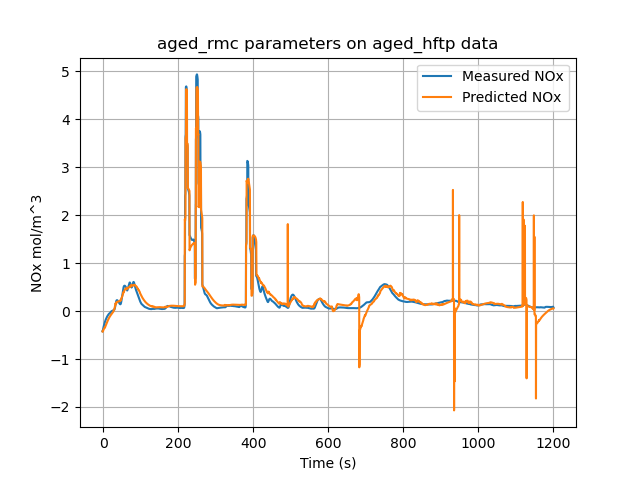
\includegraphics[width = \textwidth]{./figs/figs_new_mdl/aged_rmc_aged_hftp.png}
        \end{minipage}
        \begin{minipage}{0.3\textwidth}
                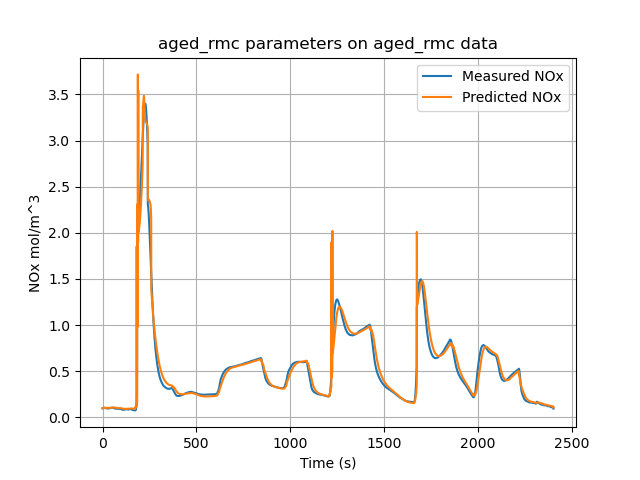
\includegraphics[width = \textwidth]{./figs/figs_new_mdl/aged_rmc_aged_rmc.png}
        \end{minipage}
        \caption{Cross validation using aged$\_$rmc parameter estimates}
\end{figure}


\subsection{Comparing Aged and Degreened parameter estimates}

\begin{figure}[H]
        \begin{minipage}{0.3\textwidth}
                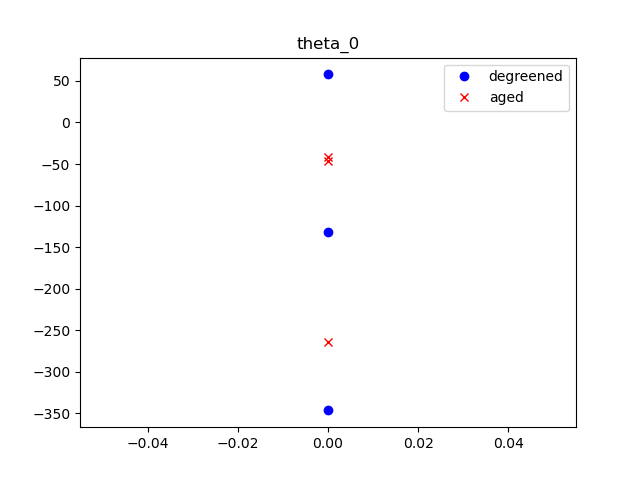
\includegraphics[width = \textwidth]{./figs/figs_new_mdl/theta_0.png}
        \end{minipage}
        \begin{minipage}{0.3\textwidth}
                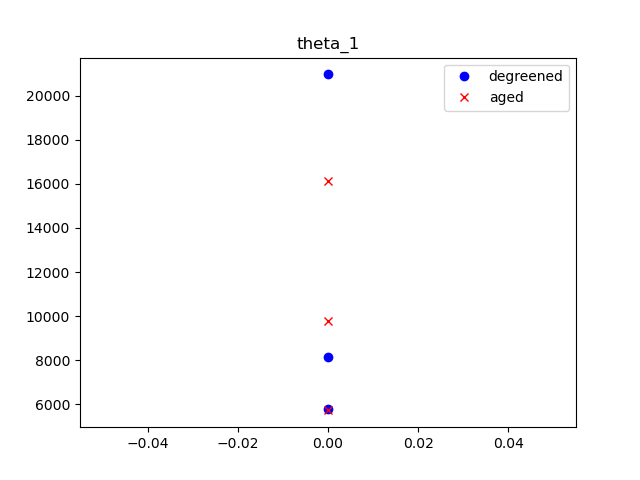
\includegraphics[width = \textwidth]{./figs/figs_new_mdl/theta_1.png}
        \end{minipage}
        \begin{minipage}{0.3\textwidth}
                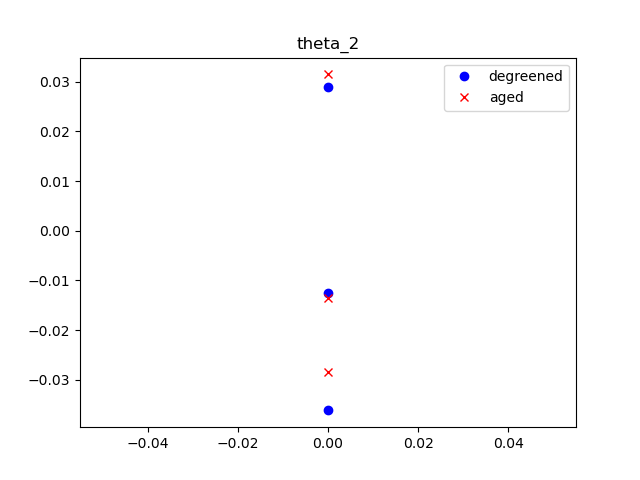
\includegraphics[width = \textwidth]{./figs/figs_new_mdl/theta_2.png}
        \end{minipage}
\end{figure}

\begin{figure}[H]
        \begin{minipage}{0.3\textwidth}
                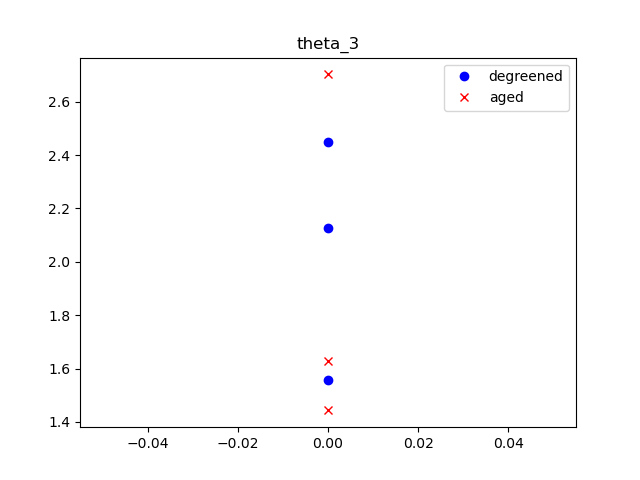
\includegraphics[width = \textwidth]{./figs/figs_new_mdl/theta_3.png}
        \end{minipage}
        \begin{minipage}{0.3\textwidth}
                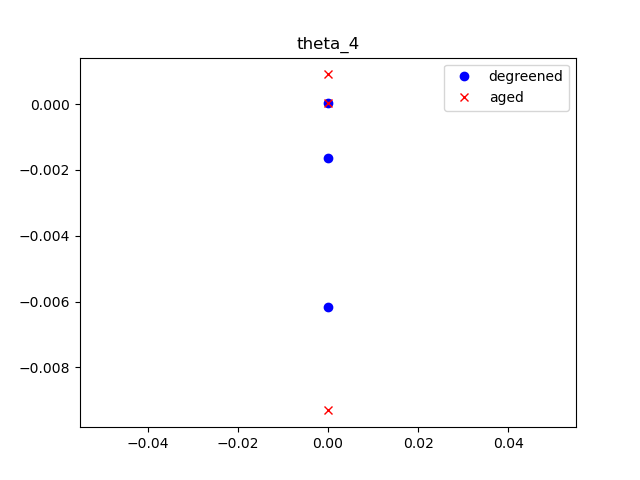
\includegraphics[width = \textwidth]{./figs/figs_new_mdl/theta_4.png}
        \end{minipage}
        \begin{minipage}{0.3\textwidth}
                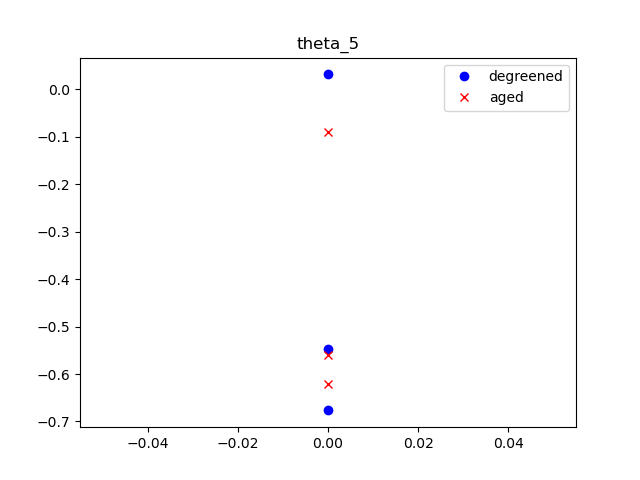
\includegraphics[width = \textwidth]{./figs/figs_new_mdl/theta_5.png}
        \end{minipage}
\end{figure}

\begin{figure}[H]
        \begin{minipage}{0.3\textwidth}
                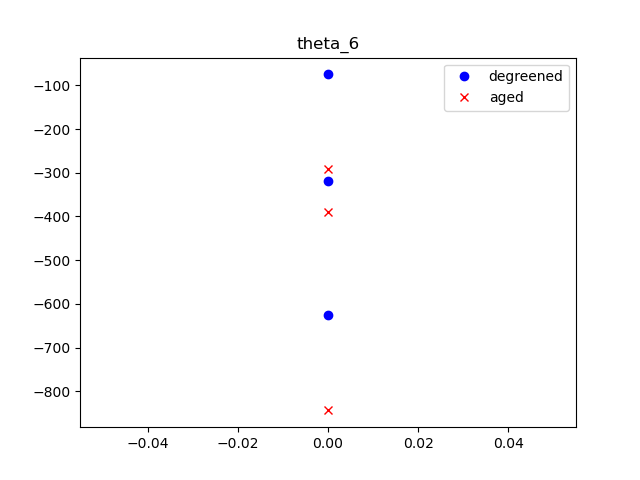
\includegraphics[width = \textwidth]{./figs/figs_new_mdl/theta_6.png}
        \end{minipage}
        \begin{minipage}{0.3\textwidth}
                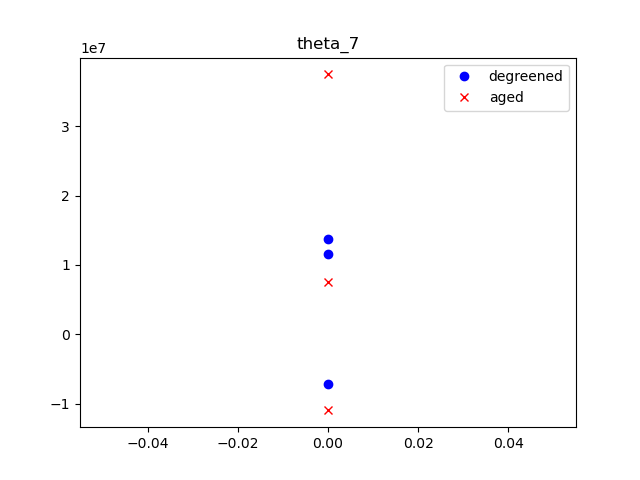
\includegraphics[width = \textwidth]{./figs/figs_new_mdl/theta_7.png}
        \end{minipage}
        \begin{minipage}{0.3\textwidth}
                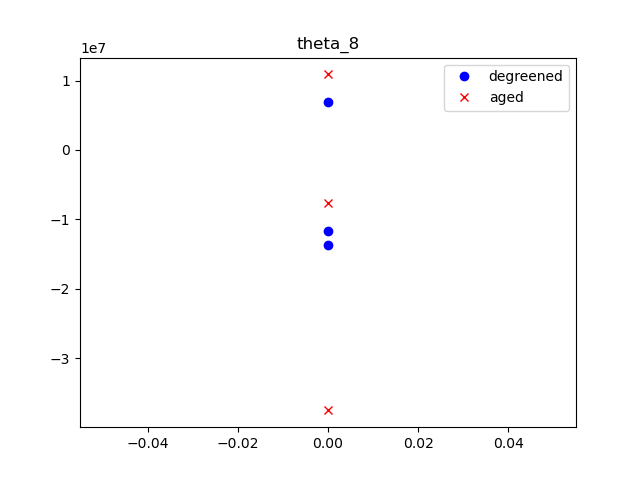
\includegraphics[width = \textwidth]{./figs/figs_new_mdl/theta_8.png}
        \end{minipage}
\end{figure}

\begin{figure}[H]
        \centering
        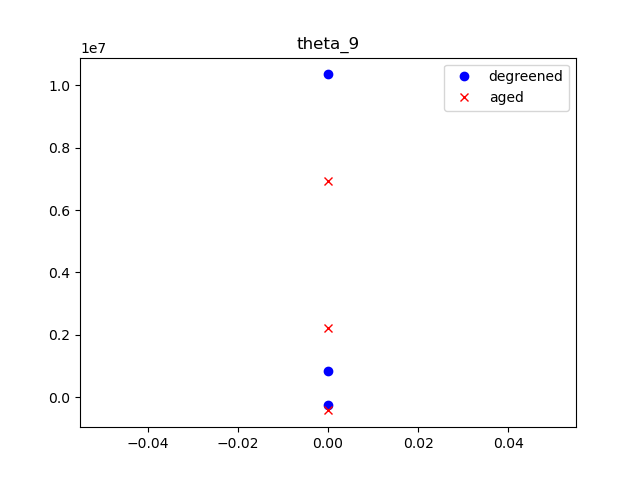
\includegraphics[width = 0.3\textwidth]{./figs/figs_new_mdl/theta_9.png}
\end{figure}

\section{Remarks}
This work developed a uniquely identifiable parametric nonlinear model structure for SCR-ASC dynamics based on the first principles. The cross-validation results show the goodness of fit for the model. The parameters are not distinct with respect to the aging of the catalyst. The parametric structure is unique while the actual parameter and regression vectors can be tweaked based on models for rate constants, residence time and urea injection. This allows us to choose appropriate assumptions for the reduced order model for the process.


\section*{List of Symbols}

\begin{table}[H]
    \small
    \begin{tabular}{r c l}
        $\lrf{\bullet}$ &$-$& Number of moles of $\bullet$. $(moles)$\\
        $\lrb{\bullet}$ &$-$& Concentration of $\bullet$. $(moles/ml = mol/cm^3)$\\
        $\Theta_{free/occupied}$ &$-$& Moles of adsorption sites free/occupied. $(moles)$\\
        $A_{scr}$ &$-$& Area of SCR catalyst bed $\lr{cm^2}$ \\
        $\Gamma $ &$-$& Surface concentration of the total storage capacity for the catalyst $(moles/cm^2)$ .\\
                  &   & $= \frac{\Theta_{free} + \Theta_{occupied}}{A_{scr}}$ \\
        $E_i$ &$-$& Activation Energy of $i^{th}$ reaction\\
        $A_i$ &$-$& Pre-exponential factor of $i^{th}$ reaction\\
        $R$ &$-$& Universal gas constant\\
        $T$ &$-$& Temperature\\
        $L$ &$-$& Length of the catalyst bed\\
        $A$ &$-$& Cross-sectional area of the catalyst chamber\\
        $V$ &$-$& Volume of the catalyst chamber\\
        $f_v$ &$-$& Volume flow rate of the exhaust gasses $(ml/s)$\\
        $F$ &$-$& Mass flow rate of the exhaust gasses $(g/s)$\\
        $\rho$ &$-$& Density of the exhaust gasses $(g/cm^3)$\\
        $\Omega(k)$ &$-$& Total change in the surface concentration of adsorbed ammonia in the sample [k] to [k+1]\\
        $\sigma(k)$ &$-$& Average surface concentration of adsorbed ammonia in the sample [k] to [k+1]\\
        $\mu$ &$-$& Average molecular weight of the exhaust gasses (Including humidity)\\
    \end{tabular}
\end{table}


\chapter{Conclusion and Future Work}













% \chapter{Survey of SCR modelling and diagnostics}
% \chapter{Residence time aware discrete-time modelling and Identification of SCR-ASC systems}
% \chapter{Aging Characterization of SCR-ASC systems}
% \chapter{Demonstration using real-world truck data from Cummins Inc.}

%%======================================================================================================================

%%======================================================================================================================
%% End Stuff
% \input{Appendices/ap0-appendices.tex}   % Appendices
% -------------------- From Template -------------------
% Currently commented out (depends on if using BibLaTeX)

%
% This is only done if you are using BibLaTeX.
%
\makeatletter  % commented out on 2022-01-26
  \defbibenvironment{bibliography}
    {%
      \list
        {%
          \printtext[labelnumberwidth]%
          {%
            \printfield{prefixnumber}%
            \printfield{labelnumber}%
          }%
        }%
        {%
          \setlength{\bibhang}{1in} %%%%% was 0pt
          \setlength{\itemindent}{1in}%  -\leftmargin} %%%%% was 0pt
          \setlength{\itemsep}{\bibitemsep}%
          \setlength{\leftmargin}{0pt}%  .22in} % 0.42in}
          \setlength{\parsep}{\bibparsep}%
           \setlength{\rightmargin}{0.33in}%
        }%
    }
    {\endlist}
    {\item}
\makeatother  % commented out on 2022-01-26



% \immediate\setlength{\labelnumberwidth}{1.5in} %%%%% was commented out
\setlength{\labelwidth}{1.5in}
\def\sllnsez{[999] }

{%
  % Make _ in URLs visible.
  % \def\t{\char'137}%
  \catcode`*=\active
  \def*{\char'137}%  \char'137 is _
  \PrintBibliography
}
              % Back content (vita, bib settings, etc.)
\end{document}
